\documentclass[review]{elsarticle}

%\modulolinenumbers[5]

\usepackage{ucs}
\usepackage[utf8x]{inputenc}
\usepackage{graphicx}
\usepackage{amsmath,amsthm}
\usepackage{amssymb}
\usepackage{url}
\usepackage{stmaryrd}
\usepackage{ifpdf, proof}
\ifpdf
  \usepackage{hyperref}
\fi
%\usepackage[x11names]{xcolor}
%\usepackage[all]{xy}
%\usepackage{xspace}
%\usepackage{pstricks}
%\usepackage{listings}
%\usepackage{wrapfig}
%\usepackage{mathpartir}

%% ODER: format ==         = "\mathrel{==}"
%% ODER: format /=         = "\neq "
%
%
\makeatletter
\@ifundefined{lhs2tex.lhs2tex.sty.read}%
  {\@namedef{lhs2tex.lhs2tex.sty.read}{}%
   \newcommand\SkipToFmtEnd{}%
   \newcommand\EndFmtInput{}%
   \long\def\SkipToFmtEnd#1\EndFmtInput{}%
  }\SkipToFmtEnd

\newcommand\ReadOnlyOnce[1]{\@ifundefined{#1}{\@namedef{#1}{}}\SkipToFmtEnd}
\usepackage{amstext}
\usepackage{amssymb}
\usepackage{stmaryrd}
\DeclareFontFamily{OT1}{cmtex}{}
\DeclareFontShape{OT1}{cmtex}{m}{n}
  {<5><6><7><8>cmtex8
   <9>cmtex9
   <10><10.95><12><14.4><17.28><20.74><24.88>cmtex10}{}
\DeclareFontShape{OT1}{cmtex}{m}{it}
  {<-> ssub * cmtt/m/it}{}
\newcommand{\texfamily}{\fontfamily{cmtex}\selectfont}
\DeclareFontShape{OT1}{cmtt}{bx}{n}
  {<5><6><7><8>cmtt8
   <9>cmbtt9
   <10><10.95><12><14.4><17.28><20.74><24.88>cmbtt10}{}
\DeclareFontShape{OT1}{cmtex}{bx}{n}
  {<-> ssub * cmtt/bx/n}{}
\newcommand{\tex}[1]{\text{\texfamily#1}}	% NEU

\newcommand{\Sp}{\hskip.33334em\relax}


\newcommand{\Conid}[1]{\mathit{#1}}
\newcommand{\Varid}[1]{\mathit{#1}}
\newcommand{\anonymous}{\kern0.06em \vbox{\hrule\@width.5em}}
\newcommand{\plus}{\mathbin{+\!\!\!+}}
\newcommand{\bind}{\mathbin{>\!\!\!>\mkern-6.7mu=}}
\newcommand{\rbind}{\mathbin{=\mkern-6.7mu<\!\!\!<}}% suggested by Neil Mitchell
\newcommand{\sequ}{\mathbin{>\!\!\!>}}
\renewcommand{\leq}{\leqslant}
\renewcommand{\geq}{\geqslant}
\usepackage{polytable}

%mathindent has to be defined
\@ifundefined{mathindent}%
  {\newdimen\mathindent\mathindent\leftmargini}%
  {}%

\def\resethooks{%
  \global\let\SaveRestoreHook\empty
  \global\let\ColumnHook\empty}
\newcommand*{\savecolumns}[1][default]%
  {\g@addto@macro\SaveRestoreHook{\savecolumns[#1]}}
\newcommand*{\restorecolumns}[1][default]%
  {\g@addto@macro\SaveRestoreHook{\restorecolumns[#1]}}
\newcommand*{\aligncolumn}[2]%
  {\g@addto@macro\ColumnHook{\column{#1}{#2}}}

\resethooks

\newcommand{\onelinecommentchars}{\quad-{}- }
\newcommand{\commentbeginchars}{\enskip\{-}
\newcommand{\commentendchars}{-\}\enskip}

\newcommand{\visiblecomments}{%
  \let\onelinecomment=\onelinecommentchars
  \let\commentbegin=\commentbeginchars
  \let\commentend=\commentendchars}

\newcommand{\invisiblecomments}{%
  \let\onelinecomment=\empty
  \let\commentbegin=\empty
  \let\commentend=\empty}

\visiblecomments

\newlength{\blanklineskip}
\setlength{\blanklineskip}{0.66084ex}

\newcommand{\hsindent}[1]{\quad}% default is fixed indentation
\let\hspre\empty
\let\hspost\empty
\newcommand{\NB}{\textbf{NB}}
\newcommand{\Todo}[1]{$\langle$\textbf{To do:}~#1$\rangle$}

\EndFmtInput
\makeatother
%
%
%
%
%
%
% This package provides two environments suitable to take the place
% of hscode, called "plainhscode" and "arrayhscode". 
%
% The plain environment surrounds each code block by vertical space,
% and it uses \abovedisplayskip and \belowdisplayskip to get spacing
% similar to formulas. Note that if these dimensions are changed,
% the spacing around displayed math formulas changes as well.
% All code is indented using \leftskip.
%
% Changed 19.08.2004 to reflect changes in colorcode. Should work with
% CodeGroup.sty.
%
\ReadOnlyOnce{polycode.fmt}%
\makeatletter

\newcommand{\hsnewpar}[1]%
  {{\parskip=0pt\parindent=0pt\par\vskip #1\noindent}}

% can be used, for instance, to redefine the code size, by setting the
% command to \small or something alike
\newcommand{\hscodestyle}{}

% The command \sethscode can be used to switch the code formatting
% behaviour by mapping the hscode environment in the subst directive
% to a new LaTeX environment.

\newcommand{\sethscode}[1]%
  {\expandafter\let\expandafter\hscode\csname #1\endcsname
   \expandafter\let\expandafter\endhscode\csname end#1\endcsname}

% "compatibility" mode restores the non-polycode.fmt layout.

\newenvironment{compathscode}%
  {\par\noindent
   \advance\leftskip\mathindent
   \hscodestyle
   \let\\=\@normalcr
   \let\hspre\(\let\hspost\)%
   \pboxed}%
  {\endpboxed\)%
   \par\noindent
   \ignorespacesafterend}

\newcommand{\compaths}{\sethscode{compathscode}}

% "plain" mode is the proposed default.
% It should now work with \centering.
% This required some changes. The old version
% is still available for reference as oldplainhscode.

\newenvironment{plainhscode}%
  {\hsnewpar\abovedisplayskip
   \advance\leftskip\mathindent
   \hscodestyle
   \let\hspre\(\let\hspost\)%
   \pboxed}%
  {\endpboxed%
   \hsnewpar\belowdisplayskip
   \ignorespacesafterend}

\newenvironment{oldplainhscode}%
  {\hsnewpar\abovedisplayskip
   \advance\leftskip\mathindent
   \hscodestyle
   \let\\=\@normalcr
   \(\pboxed}%
  {\endpboxed\)%
   \hsnewpar\belowdisplayskip
   \ignorespacesafterend}

% Here, we make plainhscode the default environment.

\newcommand{\plainhs}{\sethscode{plainhscode}}
\newcommand{\oldplainhs}{\sethscode{oldplainhscode}}
\plainhs

% The arrayhscode is like plain, but makes use of polytable's
% parray environment which disallows page breaks in code blocks.

\newenvironment{arrayhscode}%
  {\hsnewpar\abovedisplayskip
   \advance\leftskip\mathindent
   \hscodestyle
   \let\\=\@normalcr
   \(\parray}%
  {\endparray\)%
   \hsnewpar\belowdisplayskip
   \ignorespacesafterend}

\newcommand{\arrayhs}{\sethscode{arrayhscode}}

% The mathhscode environment also makes use of polytable's parray 
% environment. It is supposed to be used only inside math mode 
% (I used it to typeset the type rules in my thesis).

\newenvironment{mathhscode}%
  {\parray}{\endparray}

\newcommand{\mathhs}{\sethscode{mathhscode}}

% texths is similar to mathhs, but works in text mode.

\newenvironment{texthscode}%
  {\(\parray}{\endparray\)}

\newcommand{\texths}{\sethscode{texthscode}}

% The framed environment places code in a framed box.

\def\codeframewidth{\arrayrulewidth}
\RequirePackage{calc}

\newenvironment{framedhscode}%
  {\parskip=\abovedisplayskip\par\noindent
   \hscodestyle
   \arrayrulewidth=\codeframewidth
   \tabular{@{}|p{\linewidth-2\arraycolsep-2\arrayrulewidth-2pt}|@{}}%
   \hline\framedhslinecorrect\\{-1.5ex}%
   \let\endoflinesave=\\
   \let\\=\@normalcr
   \(\pboxed}%
  {\endpboxed\)%
   \framedhslinecorrect\endoflinesave{.5ex}\hline
   \endtabular
   \parskip=\belowdisplayskip\par\noindent
   \ignorespacesafterend}

\newcommand{\framedhslinecorrect}[2]%
  {#1[#2]}

\newcommand{\framedhs}{\sethscode{framedhscode}}

% The inlinehscode environment is an experimental environment
% that can be used to typeset displayed code inline.

\newenvironment{inlinehscode}%
  {\(\def\column##1##2{}%
   \let\>\undefined\let\<\undefined\let\\\undefined
   \newcommand\>[1][]{}\newcommand\<[1][]{}\newcommand\\[1][]{}%
   \def\fromto##1##2##3{##3}%
   \def\nextline{}}{\) }%

\newcommand{\inlinehs}{\sethscode{inlinehscode}}

% The joincode environment is a separate environment that
% can be used to surround and thereby connect multiple code
% blocks.

\newenvironment{joincode}%
  {\let\orighscode=\hscode
   \let\origendhscode=\endhscode
   \def\endhscode{\def\hscode{\endgroup\def\@currenvir{hscode}\\}\begingroup}
   %\let\SaveRestoreHook=\empty
   %\let\ColumnHook=\empty
   %\let\resethooks=\empty
   \orighscode\def\hscode{\endgroup\def\@currenvir{hscode}}}%
  {\origendhscode
   \global\let\hscode=\orighscode
   \global\let\endhscode=\origendhscode}%

\makeatother
\EndFmtInput
%

\DeclareMathAlphabet{\mathkw}{OT1}{cmss}{bx}{n}

\newtheorem{Lemma}{Lemma}
\newtheorem{Theorem}{Theorem}
\theoremstyle{definition}
\newtheorem{Example}{Example}

\usepackage{color}
\newcommand{\redFG}[1]{\textcolor[rgb]{0.6,0,0}{#1}}
\newcommand{\greenFG}[1]{\textcolor[rgb]{0,0.4,0}{#1}}
\newcommand{\blueFG}[1]{\textcolor[rgb]{0,0,0.8}{#1}}
\newcommand{\orangeFG}[1]{\textcolor[rgb]{0.8,0.4,0}{#1}}
\newcommand{\purpleFG}[1]{\textcolor[rgb]{0.4,0,0.4}{#1}}
\newcommand{\yellowFG}[1]{\textcolor{yellow}{#1}}
\newcommand{\brownFG}[1]{\textcolor[rgb]{0.5,0.2,0.2}{#1}}
\newcommand{\blackFG}[1]{\textcolor[rgb]{0,0,0}{#1}}
\newcommand{\whiteFG}[1]{\textcolor[rgb]{1,1,1}{#1}}
\newcommand{\yellowBG}[1]{\colorbox[rgb]{1,1,0.2}{#1}}
\newcommand{\brownBG}[1]{\colorbox[rgb]{1.0,0.7,0.4}{#1}}

\newcommand{\ColourStuff}{
  \newcommand{\red}{\redFG}
  \newcommand{\green}{\greenFG}
  \newcommand{\blue}{\blueFG}
  \newcommand{\orange}{\orangeFG}
  \newcommand{\purple}{\purpleFG}
  \newcommand{\yellow}{\yellowFG}
  \newcommand{\brown}{\brownFG}
  \newcommand{\black}{\blackFG}
  \newcommand{\white}{\whiteFG}
}

\newcommand{\MonochromeStuff}{
  \newcommand{\red}{\blackFG}
  \newcommand{\green}{\blackFG}
  \newcommand{\blue}{\blackFG}
  \newcommand{\orange}{\blackFG}
  \newcommand{\purple}{\blackFG}
  \newcommand{\yellow}{\blackFG}
  \newcommand{\brown}{\blackFG}
  \newcommand{\black}{\blackFG}
  \newcommand{\white}{\blackFG}
}

\ColourStuff

\newcommand{\D}[1]{\blue{\mathsf{#1}}}
\newcommand{\C}[1]{\red{\mathsf{#1}}}
\newcommand{\F}[1]{\green{\mathsf{#1}}}
\newcommand{\V}[1]{\purple{\mathit{#1}}}


\journal{Science of Computer Programming}

\bibliographystyle{elsarticle-num}

\begin{document}

\begin{frontmatter}

\title{Certified Derivative-Based Parsing of\\ Regular Expressions}

%% Group authors per affiliation:

\author[rgr]{Rodrigo Ribeiro}
\cortext[rgr]{Corresponding author}
\address{Dep. de Computa\c{c}\~ao, Universidade
Federal de Ouro Preto, ICEB, \newline Campus Universit\'ario Morro do
Cruzeiro, Ouro Preto, Minas Gerais, Brasil}
\ead{rodrigo@decsi.ufop.br}

\author{Raul Lopes}
\address{Dep. de Computa\c{c}\~ao, Universidade
  Federal de Ouro Preto, ICEB, \newline Campus Universit\'ario Morro do
  Cruzeiro, Ouro Preto, Minas Gerais, Brasil}
\ead{raulfpl@gmail.com}

\author{Carlos Camar\~ao}
\address{Dep. de Ci\^encia da Computa\c{c}\~ao, Universidade Federal
  de Minas Gerais, \newline Av. Ant\^onio Carlos 6627, Belo Horizonte, Minas Gerais, Brasil}
\ead{camarao@dcc.ufmg.br}

\begin{abstract}

We describe the formalization of Brzozowski and Antimirov derivative
based algorithms for regular expression parsing, in the dependently
typed language Agda. The formalization produces a proof that either an
input string matches a given regular expression or that no matching
exists. A tool for regular expression based search in the style of the
well known GNU grep has been developed with the certified algorithms.
Practical experiments conducted with this tool are reported.

\end{abstract}

\begin{keyword}
Certified algorithms, regular expressions; dependent types
\end{keyword}

\end{frontmatter}


\section{Introduction}\label{sec:intro}

Parsing is the process of analysing if a string of symbols conforms to
a given set of rules. It involves in computer science the formal
specification of the rules in a grammar and, also, either the
construction of data that makes evident which rules have been used to
conclude that the string of symbols can be obtained from the grammar
rules or, otherwise, an indication of an error that represents the
fact that the string of symbols cannot be generated from the grammar
rules.

In this work we are interested in the parsing problem for regular
languages (RLs)~\cite{Hopcroft2000}, i.e.~languages that can be
recognized by (non-)deterministic finite automata and equivalent
formalisms. Regular expressions (REs) are an algebraic and compact way
of specifying RLs that are extensively used in lexical analyser
generators~\cite{Lesk1990} and string search utilities~\cite{Grep}.
Since such tools are widely used and parsing is pervasive in
computing, there is a growing interest on certified parsing
algorithms~\cite{FirsovU13,Firsov14,Danielsson2010}.  This interest
is motivated by the recent development of dependently typed
languages. Such languages are powerful enough to express algorithmic
properties as types, that are automatically checked by a compiler.

The use of derivatives for regular expressions were introduced by
Brzozowski~\cite{Brzozowski1964} as an alternative method to compute a
finite state machine that is equivalent to a given RE and to perform
RE-based parsing. According to Owens et. al~\cite{Owens2009},
``derivatives have been lost in the sands of time'' until their work on
functional encoding of RE derivatives have renewed interest on their use
for parsing~\cite{Might2011,Fischer2010}.  In this work, we provide a
complete formalization of an algorithm for RE parsing using
derivatives \cite{Owens2009}, and describe a RE based search tool we developed by 
using the dependently typed language
Agda~\cite{Norell2009}. We want to emphasize that what we call ``RE parsing''
is the problem of finding all prefixes and substrings of a input that matches
a given RE, as in RE based text search tools as GNU-grep~\cite{Grep}.

More specifically, our contributions are:
\begin{itemize}
  \item A formalization of Brzozowski derivatives based RE parsing in
    Agda. The certified algorithm presented produces as a result
    either a proof term (parse tree) that is evidence that the input
    string is in the language of the input RE or a witness that such
    parse tree does not exist.

  \item A detailed explanation of the technique used to simplify
    derivatives using ``smart-constructors''~\cite{Owens2009}.
    We give formal proofs that smart constructors indeed preserve
    the language recognized by REs.

  \item A formalization of Antimirov's partial derivatives and their use to
    construct a RE parsing algorithm. The main difference between
    partial derivatives and Brzozowski's is that the former computes a
    set of REs using set operators instead of ``smart-constructors''.
    Producing a set of REs avoids the need of simplification using
    smart constructors.
\end{itemize}

This paper extends our SBLP 2016 paper~\cite{Lopes2016} by formalizing
a RE parsing algorithm using Antimirov's partial
derivatives~\cite{Antimirov1996}.  Also our original paper uses
Idris~\cite{Brady2013} instead of Agda. This change was motivated by a
modification in Idris totality checker that refuses some (correct and
total) proofs that are both accepted by Agda's and Coq totality
checkers. All source code produced in Idris, Agda and Coq, including
the \LaTeX~ source of this article, are avaliable
on-line~\cite{regex-rep}.

The rest of this paper is organized as follows. Section~\ref{sec:agda}
presents a brief introduction to Agda. Section~\ref{sec:regexp}
describes the encoding of REs and its parse trees. In
Section~\ref{sec:deriv} we define Brzozowski and Antimirov derivatives
and smart constructors, some of their properties and describe how to
build a correct parsing algorithm from them. Section~\ref{sec:exp}
comments on the use of the certified algorithm to build a tool for
RE-based search and present some experiments with this tool. Related
work is discussed on
Section~\ref{sec:related}. Section~\ref{sec:conclusion} concludes.

All the source code in this article has been formalized in Agda
version 2.5.2 using Standard Library 0.13, but
we do not present every detail. Proofs of some properties result in
functions with a long pattern matching structure, that would distract
the reader from understanding the high-level structure of the
formalization. In such situations we give just proof sketches and point
out where all details can be found in the source code.

\section{An Overview of Agda}\label{sec:agda}


Agda is a dependently-typed functional programming language based on
Martin-L\"of intuitionistic type theory~\cite{Lof98}.  Function types
and an infinite hierarchy of types, \ensuremath{\D{Set}\;\V{l}}, where \ensuremath{\V{l}} is a
natural number, are built-in. Everything else is a user-defined
type. The type \ensuremath{\D{Set}}, also known as \ensuremath{\D{Set}_{\D{0}}}, is the type of all
``small'' types, such as \ensuremath{\D{Bool}}, \ensuremath{\D{String}} and \ensuremath{\D{List}\;\D{Bool}}.  The type
\ensuremath{\D{Set}_{\D{1}}} is the type of \ensuremath{\D{Set}} and ``others like it'', such as \ensuremath{\D{Set}\;\to \;\D{Bool}}, \ensuremath{\D{String}\;\to \;\D{Set}}, and \ensuremath{\D{Set}\;\to \;\D{Set}}. We have that \ensuremath{\D{Set}\;\V{l}} is an
element of the type \ensuremath{\D{Set}\;(\V{l+1})}, for every $l≥0$. This
stratification of types is used to keep Agda consistent as a logical
theory~\cite{Sorensen2006}.

An ordinary (non-dependent) function type is written \ensuremath{\V{A}\;\to \;\V{B}} and a
dependent one is written \ensuremath{(\V{x}\;\mathbin{:}\;\V{A})\;\to \;\V{B}}, where type \ensuremath{\V{B}} depends on
\ensuremath{\V{x}}, or \ensuremath{\V{∀}\;(\V{x}\;\mathbin{:}\;\V{A})\;\to \;\V{B}}. Agda allows the definition of \emph{implicit
parameters}, i.e.  parameters whose value can be infered from the
context, by surrounding them in curly braces: \ensuremath{\V{∀}\;\{\mskip1.5mu \V{x}\;\mathbin{:}\;\V{A}\mskip1.5mu\}\;\to \;\V{B}}. To
avoid clutter, we'll omit implicit arguments from the source code
presentation. The reader can safely assume that every free variable in
a type is an implicity parameter.

As an example of Agda code, consider the the following data type of
length-indexed lists, also known as vectors.

\begin{hscode}\SaveRestoreHook
\column{B}{@{}>{\hspre}l<{\hspost}@{}}%
\column{3}{@{}>{\hspre}l<{\hspost}@{}}%
\column{5}{@{}>{\hspre}l<{\hspost}@{}}%
\column{9}{@{}>{\hspre}l<{\hspost}@{}}%
\column{E}{@{}>{\hspre}l<{\hspost}@{}}%
\>[3]{}\mathkw{data}\;\D{\mathbb{N}}\;\mathbin{:}\;\D{Set}\;\mathkw{where}{}\<[E]%
\\
\>[3]{}\hsindent{2}{}\<[5]%
\>[5]{}\C{zero}\;\mathbin{:}\;\D{\mathbb{N}}{}\<[E]%
\\
\>[3]{}\hsindent{2}{}\<[5]%
\>[5]{}\C{suc}\;\mathbin{:}\;\D{\mathbb{N}}\;\to \;\D{\mathbb{N}}{}\<[E]%
\\[\blanklineskip]%
\>[3]{}\mathkw{data}\;\D{Vec}\;(\V{A}\;\mathbin{:}\;\D{Set})\;\mathbin{:}\;\D{\mathbb{N}}\;\to \;\D{Set}\;\mathkw{where}{}\<[E]%
\\
\>[3]{}\hsindent{2}{}\<[5]%
\>[5]{}\C{\lbrack\:\rbrack}\;{}\<[9]%
\>[9]{}\mathbin{:}\;\D{Vec}\;\V{A}\;\C{zero}{}\<[E]%
\\
\>[3]{}\hsindent{2}{}\<[5]%
\>[5]{}\V{\char95 ::\char95 }\;\mathbin{:}\;\V{∀}\;\{\mskip1.5mu \V{n}\mskip1.5mu\}\;\to \;\V{A}\;\to \;\D{Vec}\;\V{A}\;\V{n}\;\to \;\D{Vec}\;\V{A}\;(\C{suc}\;\V{n}){}\<[E]%
\ColumnHook
\end{hscode}\resethooks
The \ensuremath{\D{Vec}} type uses some interesting concepts. 
First, \ensuremath{\D{Vec}} is \emph{parameterized} by a type \ensuremath{\V{A}\;\mathbin{:}\;\D{Set}}, which means that 
in every occurrence of \ensuremath{\D{Vec}} its parameter \ensuremath{\V{A}} should not change. Second, 
the type of \ensuremath{\D{Vec}\;\V{A}} is \ensuremath{\D{\mathbb{N}}\;\to \;\D{Set}}, i.e.
\ensuremath{\D{Vec}\;\V{A}} is a family of types indexed by natural numbers. 
For each natural number \ensuremath{\V{n}}, \ensuremath{\D{Vec}\;\V{A}\;\V{n}} is a type. 

In \ensuremath{\D{Vec}} definition, the constructor \ensuremath{\C{\lbrack\:\rbrack}} builds empty vectors. The cons-operator (\ensuremath{\V{\char95 ::\char95 }})
inserts a new element in front of a vector of $n$ elements (of type
\ensuremath{\D{Vec}\;\V{A}\;\V{n}}) and returns a value of type \ensuremath{\D{Vec}\;\V{A}\;(\C{suc}\;\V{n})}. The
\ensuremath{\D{Vec}} datatype is an example of a dependent type, i.e. a type
that uses a value (that denotes its length). The usefulness of
dependent types can be illustrated with the definition of a safe list
head function: \ensuremath{\F{head}} can be defined to accept only non-empty
vectors, i.e.~values of type \ensuremath{\D{Vec}\;\V{A}\;(\C{suc}\;\V{n})}.
\begin{hscode}\SaveRestoreHook
\column{B}{@{}>{\hspre}l<{\hspost}@{}}%
\column{3}{@{}>{\hspre}l<{\hspost}@{}}%
\column{E}{@{}>{\hspre}l<{\hspost}@{}}%
\>[3]{}\F{head}\;\mathbin{:}\;\D{Vec}\;\V{A}\;(\C{suc}\;\V{n})\;\to \;\V{A}{}\<[E]%
\\
\>[3]{}\F{head}\;(\V{x}\;\V{::}\;\V{xs})\;\mathrel{=}\;\V{x}{}\<[E]%
\ColumnHook
\end{hscode}\resethooks
In \ensuremath{\F{head}}'s definition, constructor \ensuremath{\C{\lbrack\:\rbrack}} is not used. The
Agda type-checker can figure out, from \ensuremath{\F{head}}'s parameter type,
that argument \ensuremath{\C{\lbrack\:\rbrack}} to \ensuremath{\F{head}} is not type-correct.


Thanks to the propositions-as-types principle\footnote{Also known as
  Curry-Howard ``isomorphism''~\cite{Sorensen2006}.} we can interpret
types as logical formulas and terms as proofs. We can encode logical
disjunction as the following Agda type:

\begin{hscode}\SaveRestoreHook
\column{B}{@{}>{\hspre}l<{\hspost}@{}}%
\column{4}{@{}>{\hspre}l<{\hspost}@{}}%
\column{6}{@{}>{\hspre}l<{\hspost}@{}}%
\column{E}{@{}>{\hspre}l<{\hspost}@{}}%
\>[4]{}\mathkw{data}\;\D{\_\lor\_}\;(\V{A}\;\V{B}\;\mathbin{:}\;\D{Set})\;\mathbin{:}\;\D{Set}\;\mathkw{where}{}\<[E]%
\\
\>[4]{}\hsindent{2}{}\<[6]%
\>[6]{}\C{inj_1}\;\mathbin{:}\;\V{A}\;\to \;\V{A}\;\D{\lor}\;\V{B}{}\<[E]%
\\
\>[4]{}\hsindent{2}{}\<[6]%
\>[6]{}\C{inj_2}\;\mathbin{:}\;\V{B}\;\to \;\V{A}\;\D{\lor}\;\V{B}{}\<[E]%
\ColumnHook
\end{hscode}\resethooks
Note that each constructor of the previous data type represent how
we can build evidence for the proposition \ensuremath{\V{A}\;\D{\lor}\;\V{B}}: using constructor
\ensuremath{\C{inj_1}} together with an evidence for \ensuremath{\V{A}} or using constructor \ensuremath{\C{inj_2}} and 
evidence for \ensuremath{\V{B}}. Intuitively, type \ensuremath{\D{\_\lor\_}} encodes the intuitionistic intepretation
of disjunction. Another important example is the
representation of equality as the following Agda type:

\begin{hscode}\SaveRestoreHook
\column{B}{@{}>{\hspre}l<{\hspost}@{}}%
\column{3}{@{}>{\hspre}l<{\hspost}@{}}%
\column{5}{@{}>{\hspre}l<{\hspost}@{}}%
\column{E}{@{}>{\hspre}l<{\hspost}@{}}%
\>[3]{}\mathkw{data}\;\D{\D{\equiv}}\;\{\mskip1.5mu \V{l}\mskip1.5mu\}\;\{\mskip1.5mu \V{A}\;\mathbin{:}\;\D{Set}\;\V{l}\mskip1.5mu\}\;(\V{x}\;\mathbin{:}\;\V{A})\;\mathbin{:}\;\V{A}\;\to \;\D{Set}\;\mathkw{where}{}\<[E]%
\\
\>[3]{}\hsindent{2}{}\<[5]%
\>[5]{}\C{refl}\;\mathbin{:}\;\V{x}\;\D{\equiv}\;\V{x}{}\<[E]%
\ColumnHook
\end{hscode}\resethooks

This type is called propositional equality. It defines that there is
a unique evidence for equality, constructor \ensuremath{\C{refl}} (for reflexivity),
that asserts that the only value equal to \ensuremath{\V{x}} is itself. Given a type \ensuremath{\V{P}},
type \ensuremath{\D{Dec}\;\V{P}} is used to build proofs that \ensuremath{\V{P}} is a
decidable proposition, i.e.~that either \ensuremath{\V{P}} or not \ensuremath{\V{P}}
holds. The decidable proposition type is defined as:
\begin{hscode}\SaveRestoreHook
\column{B}{@{}>{\hspre}l<{\hspost}@{}}%
\column{3}{@{}>{\hspre}l<{\hspost}@{}}%
\column{6}{@{}>{\hspre}l<{\hspost}@{}}%
\column{10}{@{}>{\hspre}l<{\hspost}@{}}%
\column{E}{@{}>{\hspre}l<{\hspost}@{}}%
\>[3]{}\mathkw{data}\;\D{Dec}\;(\V{P}\;\mathbin{:}\;\D{Set})\;\mathbin{:}\;\D{Set}\;\mathkw{where}{}\<[E]%
\\
\>[3]{}\hsindent{3}{}\<[6]%
\>[6]{}\C{yes}\;\mathbin{:}\;\V{P}\;\to \;\D{Dec}\;\V{P}{}\<[E]%
\\
\>[3]{}\hsindent{3}{}\<[6]%
\>[6]{}\C{no}\;{}\<[10]%
\>[10]{}\mathbin{:}\;\F{\neg}\;\V{P}\;\to \;\D{Dec}\;\V{P}{}\<[E]%
\ColumnHook
\end{hscode}\resethooks
Constructor \ensuremath{\C{yes}} stores a proof that property \ensuremath{\V{P}} holds
and constructor \ensuremath{\C{no}} an evidence that such proof is impossible. Some functions
used in our formalization use this type. The type \ensuremath{\V{¬}\;\V{P}} is an
abbreviation for \ensuremath{\V{P}\;\to \;\D{\bot}}, where
\ensuremath{\D{\bot}} is a data type with no constructors (i.e.~a data
type for which it is not possible to construct a value, which corresponds to
a false proposition).

Dependently typed pattern matching is built by using the so-called
\ensuremath{\mathkw{with}} construct, that allows for matching intermediate
values~\cite{McBride2004}. If the matched value has a dependent type,
then its result can affect the form of other values. For example,
consider the following code that defines a type for natural number
parity. If the natural number is even, it can be represented as the
sum of two equal natural numbers; if it is odd, it is equal to one
plus the sum of two equal values. Pattern matching on a value of
\ensuremath{\D{Parity}\;\V{n}} allows to discover if $n = j + j$ or $n = S (k + k)$,
for some $j$ and $k$ in each branch of \ensuremath{\mathkw{with}}.  Note that the
value of $n$ is specialized accordingly, using information ``learned''
by the type-checker.
\begin{hscode}\SaveRestoreHook
\column{B}{@{}>{\hspre}l<{\hspost}@{}}%
\column{4}{@{}>{\hspre}l<{\hspost}@{}}%
\column{9}{@{}>{\hspre}l<{\hspost}@{}}%
\column{25}{@{}>{\hspre}l<{\hspost}@{}}%
\column{35}{@{}>{\hspre}l<{\hspost}@{}}%
\column{43}{@{}>{\hspre}l<{\hspost}@{}}%
\column{E}{@{}>{\hspre}l<{\hspost}@{}}%
\>[B]{}\mathkw{data}\;\D{Parity}\;\mathbin{:}\;\D{\mathbb{N}}\;\to \;\D{Set}\;\mathkw{where}{}\<[E]%
\\
\>[B]{}\hsindent{4}{}\<[4]%
\>[4]{}\C{Even}\;\mathbin{:}\;\V{∀}\;\{\mskip1.5mu \V{n}\;\mathbin{:}\;\D{\mathbb{N}}\mskip1.5mu\}\;\to \;\D{Parity}\;(\V{n}\;\F{+}\;\V{n}){}\<[E]%
\\
\>[B]{}\hsindent{4}{}\<[4]%
\>[4]{}\C{Odd}\;{}\<[9]%
\>[9]{}\mathbin{:}\;\V{∀}\;\{\mskip1.5mu \V{n}\;\mathbin{:}\;\D{\mathbb{N}}\mskip1.5mu\}\;\to \;\D{Parity}\;(\C{suc}\;(\V{n}\;\F{+}\;\V{n})){}\<[E]%
\\[\blanklineskip]%
\>[B]{}\F{parity}\;\mathbin{:}\;(\V{n}\;\mathbin{:}\;\D{\mathbb{N}})\;\to \;\D{Parity}\;\V{n}{}\<[E]%
\\
\>[B]{}\F{parity}\;\mathrel{=}\mbox{\onelinecomment  definition omitted}{}\<[E]%
\\[\blanklineskip]%
\>[B]{}\F{natToBin}\;\mathbin{:}\;\D{\mathbb{N}}\;\to \;\D{List}\;\D{Bool}{}\<[E]%
\\
\>[B]{}\F{natToBin}\;\C{zero}\;\mathrel{=}\;\C{\lbrack\:\rbrack}{}\<[E]%
\\
\>[B]{}\F{natToBin}\;\V{k}\;\mathkw{with}\;(\F{parity}\;\V{k}){}\<[E]%
\\
\>[B]{}\hsindent{4}{}\<[4]%
\>[4]{}\F{natToBin}\;(\V{j}\;\F{+}\;\V{j})\;{}\<[25]%
\>[25]{}\mid \;\C{Even}\;\mathrel{=}\;\C{false}\;\V{::}\;\F{natToBin}\;\V{j}{}\<[E]%
\\
\>[B]{}\hsindent{4}{}\<[4]%
\>[4]{}\F{natToBin}\;(\C{suc}\;(\V{j}\;\F{+}\;\V{j}))\;\mid \;\C{Odd}\;{}\<[35]%
\>[35]{}\mathrel{=}\;\C{true}\;{}\<[43]%
\>[43]{}\V{::}\;\F{natToBin}\;\V{j}{}\<[E]%
\ColumnHook
\end{hscode}\resethooks

For further information about Agda, see~\cite{Norell2009,Stump16}.


\section{Regular Expressions}\label{sec:regexp}



Regular expressions are defined with respect to a given
alphabet. Formally, RE syntax follows the following context-free
grammar
\[
e ::= \emptyset\,\mid\,\epsilon\,\mid\,a\,\mid\,e\,e\,\mid\,e+e\,\mid\,e^{\star}
\]
where $a$ is any symbol from the underlying alphabet.
In our original Idris formalization, we described symbols of an alphabet as a natural number
in Peano notation (type \ensuremath{\D{\mathbb{N}}}), i.e.~the symbol's numeric
code. The reason for this design choice is due to the way that Idris
deals with propositional equality for primitive types, like
\ensuremath{\D{Char}}. Equalities of values of these types only reduce on
concrete primitive values; this causes computation of proofs to stop
under variables whose type is a primitive one. Thus, we decided to use
the inductive type \ensuremath{\D{\mathbb{N}}} to represent the codes of alphabet
symbols. In our Agda formalization, in contrast, we represent alphabet symbols using type \ensuremath{\D{Char}}.



Datatype \ensuremath{\D{Regex}} encodes RE syntax.

\begin{hscode}\SaveRestoreHook
\column{B}{@{}>{\hspre}l<{\hspost}@{}}%
\column{3}{@{}>{\hspre}l<{\hspost}@{}}%
\column{5}{@{}>{\hspre}l<{\hspost}@{}}%
\column{8}{@{}>{\hspre}l<{\hspost}@{}}%
\column{9}{@{}>{\hspre}l<{\hspost}@{}}%
\column{E}{@{}>{\hspre}l<{\hspost}@{}}%
\>[3]{}\mathkw{data}\;\D{Regex}\;\mathbin{:}\;\D{Set}\;\mathkw{where}{}\<[E]%
\\
\>[3]{}\hsindent{2}{}\<[5]%
\>[5]{}\C{\emptyset}\;{}\<[8]%
\>[8]{}\mathbin{:}\;\D{Regex}{}\<[E]%
\\
\>[3]{}\hsindent{2}{}\<[5]%
\>[5]{}\C{\epsilon}\;\mathbin{:}\;\D{Regex}{}\<[E]%
\\
\>[3]{}\hsindent{2}{}\<[5]%
\>[5]{}\C{\$\_}\;{}\<[9]%
\>[9]{}\mathbin{:}\;\D{Char}\;\to \;\D{Regex}{}\<[E]%
\\
\>[3]{}\hsindent{2}{}\<[5]%
\>[5]{}\C{\_∙\_}\;\mathbin{:}\;\D{Regex}\;\to \;\D{Regex}\;\to \;\D{Regex}{}\<[E]%
\\
\>[3]{}\hsindent{2}{}\<[5]%
\>[5]{}\C{\_+\_}\;\mathbin{:}\;\D{Regex}\;\to \;\D{Regex}\;\to \;\D{Regex}{}\<[E]%
\\
\>[3]{}\hsindent{2}{}\<[5]%
\>[5]{}\C{\_\star}\;{}\<[9]%
\>[9]{}\mathbin{:}\;\D{Regex}\;\to \;\D{Regex}{}\<[E]%
\ColumnHook
\end{hscode}\resethooks
Constructors \ensuremath{\C{\emptyset}} and \ensuremath{\C{\epsilon}} denote respectively the
empty language ($\emptyset$) and the empty string ($\epsilon$). Alphabet
symbols are constructed by using the \ensuremath{\C{\$}} constructor. Composite REs are
built using concatenation (\ensuremath{\C{∙}}), union (\ensuremath{\C{+}}) and
Kleene star (\ensuremath{\C{\star}}).


We define RE semantics as the inductively defined judgment $s \in e$, 
which means that string $s$ in is the language denoted by RE $e$.
\[
    \begin{array}{ccc}
        \infer[_{Eps}]{\epsilon \in \epsilon}{}
        & 
        \infer[_{Chr}]{a \in a}{}
        &
        \infer[_{Cat}]{ss' \in ee'}
                      {s \in e & s' \in e'} \\ \\
        \infer[_{Left}]{s \in e + e'}
                       {s \in e} & 
        \infer[_{Right}]{s \in e + e'}
                        {s \in e'} &
        \infer[_{StarBase}]{\epsilon \in e^\star}{} \\ \\ 
        \multicolumn{3}{c}{
            \infer[_{StarRec}]
                  {ss' \in e^\star}
                  {s \in e & s' \in e^\star}
        }
    \end{array}
\]
Rule $Eps$ specifies that only the empty string is accepted by RE $\epsilon$, while 
rule $Chr$ says that a single character string is accepted by the RE formed by this
character. The rules for concatenation and choice are straightforward. For Kleene star, 
we need two rules: the first specifies that the empty string is in the language of RE $e^\star$ and 
rule $StarRec$ says that the string $ss'$ is in the language denoted by $e^\star$ if 
$s \in e$ and $s' \in e^\star$.

\begin{Example}
    The string $aab$ is in the language of RE $(aa + b)^\star$, as the following derivation shows:
    \[
        \infer[_{StarRec}]{aab \in (aa + b)^\star}
              {
                  \infer[_{Left}]{aa \in aa + b}
                        {
                            \infer[_{Cat}]{aa \in aa}
                                  {
                                      \infer[_{Chr}]{a \in a}{} &
                                      \infer[_{Chr}]{a \in a}{}
                                  }
                        }
                  & 
                  \infer[_{StarRec}]{b \in (aa + b)^\star}
                        {
                            \infer[_{Right}]{b \in aa + b}
                                  {
                                      \infer[_{Chr}]{b \in b}{}
                                  }
                            & 
                            \infer[_{StarBase}]{\epsilon \in (aa + b)^\star}{}
                        }          
              }
    \]
\end{Example}
In our formalization, we represent strings as values of type \ensuremath{\D{List}\;\D{Char}} and we encode the RE semantics
as an inductive data type in which each constructor represents a rule for the previously defined semantics.
Agda allows the overloading of constructor names. In some cases we use the same symbol for 
the RE syntax and its underlying semantics.

\begin{hscode}\SaveRestoreHook
\column{B}{@{}>{\hspre}l<{\hspost}@{}}%
\column{3}{@{}>{\hspre}l<{\hspost}@{}}%
\column{5}{@{}>{\hspre}l<{\hspost}@{}}%
\column{9}{@{}>{\hspre}l<{\hspost}@{}}%
\column{29}{@{}>{\hspre}l<{\hspost}@{}}%
\column{47}{@{}>{\hspre}l<{\hspost}@{}}%
\column{E}{@{}>{\hspre}l<{\hspost}@{}}%
\>[3]{}\mathkw{data}\;\D{\_\in\llbracket\_\rrbracket}\;\mathbin{:}\;\D{List}\;\D{Char}\;\to \;\D{Regex}\;\to \;\D{Set}\;\mathkw{where}{}\<[E]%
\\
\>[3]{}\hsindent{2}{}\<[5]%
\>[5]{}\C{\epsilon}\;\mathbin{:}\;\C{\lbrack\:\rbrack}\;\D{\in\llbracket}\;\C{\epsilon}\;\D{\rrbracket}{}\<[E]%
\\
\>[3]{}\hsindent{2}{}\<[5]%
\>[5]{}\C{\$\_}\;{}\<[9]%
\>[9]{}\mathbin{:}\;(\V{a}\;\mathbin{:}\;\D{Char})\;\to \;[\mskip1.5mu \;\V{a}\;\mskip1.5mu]\;\D{\in\llbracket}\;\C{\$}\;\V{a}\;\D{\rrbracket}{}\<[E]%
\\
\>[3]{}\hsindent{2}{}\<[5]%
\>[5]{}\C{\_∙\_\Rightarrow\_}\;\mathbin{:}\;\V{xs}\;\D{\in\llbracket}\;\V{l}\;\D{\rrbracket}\;{}\<[29]%
\>[29]{}\to \;\V{ys}\;\D{\in\llbracket}\;\V{r}\;\D{\rrbracket}\;{}\<[47]%
\>[47]{}\to \;\V{zs}\;\D{\equiv}\;\V{xs}\;\F{++}\;\V{ys}\;\to \;\V{zs}\;\D{\in\llbracket}\;\V{l}\;\C{∙}\;\V{r}\;\D{\rrbracket}{}\<[E]%
\\
\>[3]{}\hsindent{2}{}\<[5]%
\>[5]{}\C{\_+L\_}\;\mathbin{:}\;(\V{r}\;\mathbin{:}\;\D{Regex})\;\to \;\V{xs}\;\D{\in\llbracket}\;\V{l}\;\D{\rrbracket}\;\to \;\V{xs}\;\D{\in\llbracket}\;\V{l}\;\C{+}\;\V{r}\;\D{\rrbracket}{}\<[E]%
\\
\>[3]{}\hsindent{2}{}\<[5]%
\>[5]{}\C{\_+R\_}\;\mathbin{:}\;(\V{l}\;\mathbin{:}\;\D{Regex})\;\to \;\V{xs}\;\D{\in\llbracket}\;\V{r}\;\D{\rrbracket}\;\to \;\V{xs}\;\D{\in\llbracket}\;\V{l}\;\C{+}\;\V{r}\;\D{\rrbracket}{}\<[E]%
\\
\>[3]{}\hsindent{2}{}\<[5]%
\>[5]{}\C{\_\star}\;\mathbin{:}\;\V{xs}\;\D{\in\llbracket}\;\C{\epsilon}\;\C{+}\;(\V{e}\;\C{∙}\;\V{e}\;\C{\star})\;\D{\rrbracket}\;\to \;\V{xs}\;\D{\in\llbracket}\;\V{e}\;\C{\star}\;\D{\rrbracket}{}\<[E]%
\ColumnHook
\end{hscode}\resethooks

Constructor \ensuremath{\C{\epsilon}} states that the empty string (denoted by the empty list \ensuremath{\C{\lbrack\:\rbrack}})
is in the language of RE \ensuremath{\C{\epsilon}}.

For any single character \ensuremath{\V{a}}, the singleton
string \ensuremath{[\mskip1.5mu \;\V{a}\;\mskip1.5mu]} is in the RL
for \ensuremath{\C{\$}\;\V{a}}. Given parse trees for REs
\ensuremath{\V{l}} and \ensuremath{\V{r}}, \ensuremath{\V{xs}\;\D{\in\llbracket}\;\V{l}\;\D{\rrbracket}} and \ensuremath{\V{ys}\;\D{\in\llbracket}\;\V{r}\;\D{\rrbracket}}, constructor
\ensuremath{\C{\_∙\_\Rightarrow\_}} can be used to build a parse tree
for the concatenation of these REs.  Constructor
\ensuremath{\C{\_+L\_}} (\ensuremath{\C{\_+R\_}}) creates a parse tree
for \ensuremath{\V{l}\;\C{+}\;\V{r}} from a parse tree for \ensuremath{\V{l}} (\ensuremath{\V{r}}). Parse trees for Kleene star
are built using the following well known equivalence of REs: $e^\star
= \epsilon + e\,e^\star$.

Several inversion lemmas about RE parsing relation are necessary for
derivative-based parsing formalization. They consist of
pattern-matching on proofs of
\ensuremath{\D{\_\in\llbracket\_\rrbracket}}. As an example, below we present the inversion 
lemma for choice operator.

\begin{hscode}\SaveRestoreHook
\column{B}{@{}>{\hspre}l<{\hspost}@{}}%
\column{3}{@{}>{\hspre}l<{\hspost}@{}}%
\column{E}{@{}>{\hspre}l<{\hspost}@{}}%
\>[3]{}\F{+invert}\;\mathbin{:}\;\V{∀}\;\{\mskip1.5mu \V{xs}\;\V{l}\;\V{r}\mskip1.5mu\}\;\V{→}\;\V{xs}\;\D{\in\llbracket}\;\V{l}\;\C{+}\;\V{r}\;\D{\rrbracket}\;\V{→}\;\V{xs}\;\D{\in\llbracket}\;\V{l}\;\D{\rrbracket}\;\D{\lor}\;\V{xs}\;\D{\in\llbracket}\;\V{r}\;\D{\rrbracket}{}\<[E]%
\\
\>[3]{}\F{+invert}\;(\V{r}\;\C{+L}\;\V{pr})\;\mathrel{=}\;\C{inj_1}\;\V{pr}{}\<[E]%
\\
\>[3]{}\F{+invert}\;(\V{l}\;\C{+R}\;\V{pr})\;\mathrel{=}\;\C{inj_2}\;\V{pr}{}\<[E]%
\ColumnHook
\end{hscode}\resethooks


Intuitively, function \ensuremath{\F{+invert}} specifies that if is the case that \ensuremath{\V{xs}\;\D{\in\llbracket}\;\V{l}\;\C{+}\;\V{r}\;\D{\rrbracket}} then
the string \ensuremath{\V{xs}} matches the RE \ensuremath{\V{l}} or it matches the RE \ensuremath{\V{r}}. Another inversion lemma 
(function \ensuremath{\F{charInvert}}) specifies that 
if a string \ensuremath{\V{x}\;\C{::}\;\V{xs}} matches the RE \ensuremath{\C{\$}\;\V{y}} then the input string must be a single character string, 
i.e. \ensuremath{\V{xs}\;\D{\equiv}\;\C{\lbrack\:\rbrack}} and \ensuremath{\V{x}\;\D{\equiv}\;\V{y}}.

\begin{hscode}\SaveRestoreHook
\column{B}{@{}>{\hspre}l<{\hspost}@{}}%
\column{3}{@{}>{\hspre}l<{\hspost}@{}}%
\column{E}{@{}>{\hspre}l<{\hspost}@{}}%
\>[3]{}\F{charInvert}\;\mathbin{:}\;\V{∀}\;\{\mskip1.5mu \V{x}\;\V{y}\;\V{xs}\mskip1.5mu\}\;\V{→}\;\V{x}\;\C{::}\;\V{xs}\;\D{\in\llbracket}\;\C{\$}\;\V{y}\;\D{\rrbracket}\;\V{→}\;\V{x}\;\D{\equiv}\;\V{y}\;\D{\times}\;\V{xs}\;\D{\equiv}\;\C{\lbrack\:\rbrack}{}\<[E]%
\\
\>[3]{}\F{charInvert}\;(\C{\$}\;\V{c})\;\mathrel{=}\;\C{refl}\;\red{,}\,\;\C{refl}{}\<[E]%
\ColumnHook
\end{hscode}\resethooks

In our formalization we have define other inversions lemmas for RE semantics relation. They follow the same
structure of the previously defined lemmas --- they produce, as result, the necessary conditions for a RE semantics 
proof to hold --- and are omitted for brevity.

\section{Derivatives, Smart Constructors and Parsing}\label{sec:deriv}

Formally, the derivative of a formal language $L\subseteq
\Sigma^\star$ with respect to a symbol $a\in\Sigma$ is the language
formed by suffixes of $L$ words without the prefix $a$.

An algorithm for computing the derivative of a language represented by
a RE as another RE is due to Brzozowski~\cite{Brzozowski1964}. It
relies on a function (called $\nu$) that determines if some RE accepts
or not the empty string (by returning \ensuremath{\C{\epsilon}} or \ensuremath{\C{\emptyset}}, respectively):
\[
    \begin{array}{lcl}
         \nu(\emptyset) & = & \emptyset \\
         \nu(\epsilon)    & = & \epsilon \\
         \nu(a)                & = & \emptyset \\
         \nu(e\,e')           & = & \left\{
                                                 \begin{array}{ll}
                                                      \epsilon &
                                                                 \text{if
                                                                 }\nu(e)
                                                                 =
                                                                 \nu(e')
                                                                 =
                                                                 \epsilon
                                                   \\
                                                   \emptyset &
                                                               \text{otherwise}
                                                 \end{array}
                                             \right. \\
         \nu(e + e')  & = & \left\{
                                         \begin{array}{ll}
                                              \epsilon & \text{if
                                                         }\nu(e) =
                                                         \epsilon
                                                         \text{ or
                                                         }\nu(e') =
                                                         \epsilon \\
                                              \emptyset & \text{otherwise}
                                         \end{array}
                                      \right. \\
         \nu(e^\star) & = & \epsilon
    \end{array}
\]
Decidability of $\nu(e)$ is proved by function \ensuremath{\F{\nu[\_]}},
which is defined by induction over the structure of the input RE
\ensuremath{\V{e}} and returns a proof that the empty string is accepted or
not, using Agda type of decidable propositions, \ensuremath{\D{Dec}\;\V{P}}.
\begin{hscode}\SaveRestoreHook
\column{B}{@{}>{\hspre}l<{\hspost}@{}}%
\column{3}{@{}>{\hspre}l<{\hspost}@{}}%
\column{E}{@{}>{\hspre}l<{\hspost}@{}}%
\>[3]{}\F{\nu[\_]}\;\mathbin{:}\;\V{∀}\;(\V{e}\;\mathbin{:}\;\D{Regex})\;\V{→}\;\D{Dec}\;(\C{\lbrack\:\rbrack}\;\D{\in\llbracket}\;\V{e}\;\D{\rrbracket}){}\<[E]%
\\
\>[3]{}\F{\nu[ }\;\C{\emptyset}\;\F{]}\;\mathrel{=}\;\C{no}\;(\lambda \;()){}\<[E]%
\\
\>[3]{}\F{\nu[ }\;\C{\epsilon}\;\F{]}\;\mathrel{=}\;\C{yes}\;\C{\epsilon}{}\<[E]%
\\
\>[3]{}\F{\nu[ }\;\C{\$}\;\V{x}\;\F{]}\;\mathrel{=}\;\C{no}\;(\lambda \;()){}\<[E]%
\\
\>[3]{}\F{\nu[ }\;\V{e}\;\C{∙}\;\V{e'}\;\F{]}\;\mathkw{with}\;\F{\nu[ }\;\V{e}\;\F{]}\;\mid \;\F{\nu[ }\;\V{e'}\;\F{]}{}\<[E]%
\\
\>[3]{}\F{\nu[ }\;\V{e}\;\C{∙}\;\V{e'}\;\F{]}\;\mid \;\C{yes}\;\V{pr}\;\mid \;(\C{yes}\;\V{pr1})\;\mathrel{=}\;\C{yes}\;(\V{pr}\;\C{∙}\;\V{pr1}\;\V{⇒}\;\C{refl}){}\<[E]%
\\
\>[3]{}\F{\nu[ }\;\V{e}\;\C{∙}\;\V{e'}\;\F{]}\;\mid \;\C{yes}\;\V{pr}\;\mid \;(\C{no}\;\V{¬pr1})\;\mathrel{=}\;\C{no}\;(\V{¬pr1}\;\V{∘}\;\F{\pi_2}\;\V{∘}\;\F{∙invert}){}\<[E]%
\\
\>[3]{}\F{\nu[ }\;\V{e}\;\C{∙}\;\V{e'}\;\F{]}\;\mid \;\C{no}\;\V{¬pr}\;\mid \;\V{pr1}\;\mathrel{=}\;\C{no}\;(\V{¬pr}\;\V{∘}\;\F{\pi_1}\;\V{∘}\;\F{∙invert}){}\<[E]%
\\
\>[3]{}\F{\nu[ }\;\V{e}\;\C{+}\;\V{e'}\;\F{]}\;\mathkw{with}\;\F{\nu[ }\;\V{e}\;\F{]}\;\mid \;\F{\nu[ }\;\V{e'}\;\F{]}{}\<[E]%
\\
\>[3]{}\F{\nu[ }\;\V{e}\;\C{+}\;\V{e'}\;\F{]}\;\mid \;\C{yes}\;\V{pr}\;\mid \;\V{pr1}\;\mathrel{=}\;\C{yes}\;(\V{e'}\;\C{+L}\;\V{pr}){}\<[E]%
\\
\>[3]{}\F{\nu[ }\;\V{e}\;\C{+}\;\V{e'}\;\F{]}\;\mid \;\C{no}\;\V{¬pr}\;\mid \;(\C{yes}\;\V{pr1})\;\mathrel{=}\;\C{yes}\;(\V{e}\;\C{+R}\;\V{pr1}){}\<[E]%
\\
\>[3]{}\F{\nu[ }\;\V{e}\;\C{+}\;\V{e'}\;\F{]}\;\mid \;\C{no}\;\V{¬pr}\;\mid \;(\C{no}\;\V{¬pr1})\;\mathrel{=}\;\C{no}\;([\mskip1.5mu \;\V{¬pr}\;\red{,}\,\;\V{¬pr1}\;\mskip1.5mu]\;\V{∘}\;\F{+invert}){}\<[E]%
\\
\>[3]{}\F{\nu[ }\;\V{e}\;\C{\star}\;\F{]}\;\mathrel{=}\;\C{yes}\;((\V{e}\;\C{∙}\;\V{e}\;\C{\star}\;\C{+L}\;\C{\epsilon})\;\C{\star}){}\<[E]%
\ColumnHook
\end{hscode}\resethooks
The definition of \ensuremath{\F{\nu[\_]}} uses some of the inversion lemmas about
RE semantics. Lemma \ensuremath{\F{∙invert}} states that if the empty string
is in the language of \ensuremath{\V{l}\;\C{∙}\;\V{r}} (where \ensuremath{\V{l}} and \ensuremath{\V{r}} are arbitrary REs)
then the empty string belongs to \ensuremath{\V{l}} and \ensuremath{\V{r}}'s languages.
Lemma \ensuremath{\F{+invert}} is defined similarly for union.

\subsection{Smart Constructors}\label{sec:smart}

In order to define Brzozowski derivatives, we follow Owens et. al.~\cite{Owens2009}. We use
smart constructors to identify equivalent REs modulo identity and nullable
elements, $\epsilon$ and $\emptyset$, respectively. RE equivalence is
denoted by $e \approx e'$ and it's defined as usual~\cite{Hopcroft2000}.
The equivalence axioms maintained by smart constructors are:
\begin{itemize}
    \item For union:
      \[
          \begin{array}{ccc}
              1)\: e + \emptyset \approx e &\hspace{1cm} & 2)\: \emptyset + e \approx e
          \end{array}
      \]
      \item For concatenation:
      \[
          \begin{array}{ccc}
              1)\: e\:\emptyset \approx \emptyset & \hspace{1cm} & 2)\: e\:\epsilon \approx e\\
              3)\: \emptyset\:e\approx \emptyset & & 4)\: \epsilon\: e \approx e\\
          \end{array}
      \]
      \item For Kleene star:
      \[
           \begin{array}{ccc}
               1)\: \emptyset^\star \approx \epsilon & \hspace{1cm} & 2)\: \epsilon^\star
                                                  \approx \epsilon
           \end{array}
      \]
\end{itemize}

These axioms are kept as invariants using functions that preserve them
while building REs. As a convention, we name smart constructors by 
prefixing a back quote to the constructor name. For union, we just need to worry when one
parameter denotes the empty language:
\begin{hscode}\SaveRestoreHook
\column{B}{@{}>{\hspre}l<{\hspost}@{}}%
\column{3}{@{}>{\hspre}l<{\hspost}@{}}%
\column{11}{@{}>{\hspre}l<{\hspost}@{}}%
\column{E}{@{}>{\hspre}l<{\hspost}@{}}%
\>[3]{}\F{\_`+\_}\;\mathbin{:}\;(\V{e}\;\V{e'}\;\mathbin{:}\;\D{Regex})\;\V{→}\;\D{Regex}{}\<[E]%
\\
\>[3]{}\C{\emptyset}\;\F{`+}\;\V{e'}\;\mathrel{=}\;\V{e'}{}\<[E]%
\\
\>[3]{}\V{e}\;\F{`+}\;\C{\emptyset}\;{}\<[11]%
\>[11]{}\mathrel{=}\;\V{e}{}\<[E]%
\\
\>[3]{}\V{e}\;\F{`+}\;\V{e'}\;\mathrel{=}\;\V{e}\;\C{+}\;\V{e'}{}\<[E]%
\ColumnHook
\end{hscode}\resethooks
In concatenation, we need to deal with the possibility of parameters
being empty (denoting the empty language) or the empty string. If one
of them is empty (\ensuremath{\C{\emptyset}}) the result is also empty. Since the empty string
is the identity for concatenation, the other parameter is returned.
\begin{hscode}\SaveRestoreHook
\column{B}{@{}>{\hspre}l<{\hspost}@{}}%
\column{3}{@{}>{\hspre}l<{\hspost}@{}}%
\column{E}{@{}>{\hspre}l<{\hspost}@{}}%
\>[3]{}\F{\_`∙\_}\;\mathbin{:}\;(\V{e}\;\V{e'}\;\mathbin{:}\;\D{Regex})\;\to \;\D{Regex}{}\<[E]%
\\
\>[3]{}\C{\emptyset}\;\F{`∙}\;\V{e'}\;\mathrel{=}\;\C{\emptyset}{}\<[E]%
\\
\>[3]{}\C{\epsilon}\;\F{`∙}\;\V{e'}\;\mathrel{=}\;\V{e'}{}\<[E]%
\\
\>[3]{}\V{e}\;\F{`∙}\;\C{\emptyset}\;\mathrel{=}\;\C{\emptyset}{}\<[E]%
\\
\>[3]{}\V{e}\;\F{`∙}\;\C{\epsilon}\;\mathrel{=}\;\V{e}{}\<[E]%
\\
\>[3]{}\V{e}\;\F{`∙}\;\V{e'}\;\mathrel{=}\;\V{e}\;\C{∙}\;\V{e'}{}\<[E]%
\ColumnHook
\end{hscode}\resethooks
For Kleene star both \ensuremath{\C{\emptyset}} and \ensuremath{\C{\epsilon}} are replaced by \ensuremath{\C{\epsilon}}.
\begin{hscode}\SaveRestoreHook
\column{B}{@{}>{\hspre}l<{\hspost}@{}}%
\column{3}{@{}>{\hspre}l<{\hspost}@{}}%
\column{E}{@{}>{\hspre}l<{\hspost}@{}}%
\>[3]{}\F{\_`⋆}\;\mathbin{:}\;\D{Regex}\;\V{→}\;\D{Regex}{}\<[E]%
\\
\>[3]{}\C{\emptyset}\;\F{`⋆}\;\mathrel{=}\;\C{\epsilon}{}\<[E]%
\\
\>[3]{}\C{\epsilon}\;\F{`⋆}\;\mathrel{=}\;\C{\epsilon}{}\<[E]%
\\
\>[3]{}\V{e}\;\F{`⋆}\;\mathrel{=}\;\V{e}\;\C{\star}{}\<[E]%
\ColumnHook
\end{hscode}\resethooks
Since all smart constructors produce equivalent REs, they preserve the
parsing relation. This property is stated below as a soundness and
completeness lemma of each smart constructor with respect to RE
membership proofs.
\begin{Lemma}[Soundness and completeness of union]
For all REs \ensuremath{\V{e}}, \ensuremath{\V{e'}} and all strings \ensuremath{\V{xs}},
\ensuremath{\V{xs}\;\D{\in\llbracket}\;\V{e}\;\F{`+}\;\V{e'}\;\D{\rrbracket}} holds if and only if, \ensuremath{\V{xs}\;\D{\in\llbracket}\;\V{e}\;\C{+}\;\V{e'}\;\D{\rrbracket}} also holds.
\end{Lemma}
\begin{proof}
  \begin{itemize}
      \item[]
      \item[($\to$)]: By case analysis on the structure of \ensuremath{\V{e}} and \ensuremath{\V{e'}}. The
  only interesting cases are when one of the expressions is
  \ensuremath{\C{\emptyset}}. If \ensuremath{\V{e}\;\mathrel{=}\;\C{\emptyset}}, then \ensuremath{\C{\emptyset}\;\F{`+}\;\V{e'}\;\mathrel{=}\;\V{e'}} and
  the desired result follows. The same reasoning applies for \ensuremath{\V{e'}\;\mathrel{=}\;\C{\emptyset}}.
      \item[($\leftarrow$)]: By case analysis on the structure of \ensuremath{\V{e}}, \ensuremath{\V{e'}}. The
   only interesting cases are when one of the REs is \ensuremath{\C{\emptyset}}.  If
   \ensuremath{\V{e}\;\mathrel{=}\;\C{\emptyset}}, we need to analyse the structure of
   \ensuremath{\V{xs}\;\D{\in\llbracket}\;\V{e}\;\C{+}\;\V{e'}\;\D{\rrbracket}}. The result follows directly or by
   contradiction using \ensuremath{\V{xs}\;\D{\in\llbracket}\;\C{\emptyset}\;\D{\rrbracket}}. The same reasoning
   applies when \ensuremath{\V{e'}\;\mathrel{=}\;\C{\emptyset}}.
  \end{itemize}          
\end{proof}
\begin{Lemma}[Soundness and completeness of concatenation]
For all REs \ensuremath{\V{e}}, \ensuremath{\V{e'}} and all strings \ensuremath{\V{xs}},
\ensuremath{\V{xs}\;\D{\in\llbracket}\;\V{e}\;\F{`∙}\;\V{e'}\;\D{\rrbracket}} holds if and only if, \ensuremath{\V{xs}\;\D{\in\llbracket}\;\V{e}\;\C{∙}\;\V{e'}\;\D{\rrbracket}}
also holds.
\end{Lemma}
\begin{proof}
    \item[]
    \item[($\to$)]:
  By case analysis on the structure of \ensuremath{\V{e}}, \ensuremath{\V{e'}}. The
  interesting cases are when \ensuremath{\V{e}} or \ensuremath{\V{e'}} are equal to
  \ensuremath{\C{\epsilon}} or \ensuremath{\C{\emptyset}}. When some of the REs are equal to
  \ensuremath{\C{\emptyset}}, the result follows by contradiction. If one of the REs
  are equal to \ensuremath{\C{\epsilon}} the desired result is immediate, from the
  proof term \ensuremath{\V{xs}\;\D{\in\llbracket}\;\V{e}\;\F{`∙}\;\V{e'}\;\D{\rrbracket}}, using list concatenation
  properties.
  \item[($\leftarrow$)]:
  By case analysis on the structure of \ensuremath{\V{e}}, \ensuremath{\V{e'}}. The
  interesting cases are when \ensuremath{\V{e}} or \ensuremath{\V{e'}} are equal to
  \ensuremath{\C{\epsilon}} or \ensuremath{\C{\emptyset}}. When some of the REs are equal to
  \ensuremath{\C{\emptyset}}, the result follows by contradiction. If one of the REs
  are equal to \ensuremath{\C{\epsilon}} the desired result is immediate.
\end{proof}  
\begin{Lemma}[Soundness and completeness of Kleene star]
For all REs \ensuremath{\V{e}} and string \ensuremath{\V{xs}},
\ensuremath{\V{xs}\;\D{\in\llbracket}\;\V{e}\;\F{`⋆}\;\D{\rrbracket}} holds if and only if, \ensuremath{\V{xs}\;\D{\in\llbracket}\;\V{e}\;\C{\star}\;\D{\rrbracket}} also holds.
\end{Lemma}
\begin{proof}
  Both directions follows by straightforward case analysis on \ensuremath{\V{e}}'s structure.
\end{proof}

All definitions of smart constructors and their properties are
contained in \texttt{Smart.agda}, in the project's on-line
repository~\cite{regex-rep}.

\subsection{Brzozowski Derivatives and their Properties}

Intuitively, the derivative of a language $L$ w.r.t. a symbol $a$, $L_a$, is the 
set of strings generated by stripping the leading $a$ from the strings in $L$
that start with $a$. Formally:  
\[
   L_a = \{ w \,\mid\, aw \in L \}
\]
Regular languages are closed under the derivative operation and Janusz Brzozowski defined a
elegant method for computing derivatives for RE in~\cite{Brzozowski1964}. 
Formally, the derivative of a RE $e$ with respect to a symbol $a$, denoted by
$\partial_a(e)$, is defined by recursion on $e$'s structure as
follows:

\[
\begin{array}{lclr}
  \partial_a(\emptyset) & = & \emptyset\\
  \partial_a(\epsilon) & = & \emptyset \\
  \partial_a(b) & = & \left\{
                      \begin{array}{lr}
                        \epsilon & \text{if } b = a\\
                        \emptyset & \text{otherwise}
                      \end{array}
                                \right. \\
  \partial_a(e\:e') & = & \partial_a(e)\,e' + \nu(e)\,\partial_a(e')\\
  \partial_a(e + e') & = & \partial_a(e) + \partial_a(e') \\
  \partial_a(e^\star) & = & \partial_a(e)\,e^\star\\
\end{array}
\]

\begin{Example}
    Consider the RE $e = (aa + b)^\star$. The derivative of $e$ w.r.t. $a$ is $a(aa + b)^\star$, as demonstrated below:
    \begin{align*}
        \partial_a((aa + b)^\star) &= \partial_a(aa + b)\,(aa + b)^\star\\ 
                                   &= \left\lbrack \partial_a (aa) + \partial_a(b)\right\rbrack\,(aa + b)^\star\\
                                   &= \left\lbrack a + \emptyset \right\rbrack\, (aa + b)^\star \\
                                   &= a(aa + b)^\star
    \end{align*}
\end{Example}    


This function has an immediate translation to Agda. Notice that the
derivative function uses smart constructors to quotient result REs
with respect to the equivalence axioms presented in
Section~\ref{sec:smart} and RE emptiness test. In the symbol case
(constructor \ensuremath{\C{\$\_}}), function \ensuremath{\F{\overset{?}{=}}} is used, which
produces an evidence for equality of two \ensuremath{\D{Char}} values.
\begin{hscode}\SaveRestoreHook
\column{B}{@{}>{\hspre}l<{\hspost}@{}}%
\column{3}{@{}>{\hspre}l<{\hspost}@{}}%
\column{E}{@{}>{\hspre}l<{\hspost}@{}}%
\>[3]{}\F{∂[\_,\_]}\;\mathbin{:}\;\D{Regex}\;\V{→}\;\D{Char}\;\V{→}\;\D{Regex}{}\<[E]%
\\
\>[3]{}\F{∂[}\;\C{\emptyset}\;\red{,}\,\;\V{c}\;\F{]}\;\mathrel{=}\;\C{\emptyset}{}\<[E]%
\\
\>[3]{}\F{∂[}\;\C{\epsilon}\;\red{,}\,\;\V{c}\;\F{]}\;\mathrel{=}\;\C{\emptyset}{}\<[E]%
\\
\>[3]{}\F{∂[}\;\C{\$}\;\V{c}\;\red{,}\,\;\V{c'}\;\F{]}\;\mathkw{with}\;\V{c}\;\F{\overset{?}{=}}\;\V{c'}{}\<[E]%
\\
\>[3]{}\V{...|}\;\C{yes}\;\C{refl}\;\mathrel{=}\;\C{\epsilon}{}\<[E]%
\\
\>[3]{}\V{...|}\;\C{no}\;\V{prf}\;\mathrel{=}\;\C{\emptyset}{}\<[E]%
\\
\>[3]{}\F{∂[}\;\V{e}\;\C{∙}\;\V{e'}\;\red{,}\,\;\V{c}\;\F{]}\;\mathkw{with}\;\F{\nu[ }\;\V{e}\;\F{]}{}\<[E]%
\\
\>[3]{}\F{∂[}\;\V{e}\;\C{∙}\;\V{e'}\;\red{,}\,\;\V{c}\;\F{]}\;\mid \;\C{yes}\;\V{pr}\;\mathrel{=}\;(\F{∂[}\;\V{e}\;\red{,}\,\;\V{c}\;\F{]}\;\F{`∙}\;\V{e'})\;\F{`+}\;\F{∂[}\;\V{e'}\;\red{,}\,\;\V{c}\;\F{]}{}\<[E]%
\\
\>[3]{}\F{∂[}\;\V{e}\;\C{∙}\;\V{e'}\;\red{,}\,\;\V{c}\;\F{]}\;\mid \;\C{no}\;\V{¬pr}\;\mathrel{=}\;\F{∂[}\;\V{e}\;\red{,}\,\;\V{c}\;\F{]}\;\F{`∙}\;\V{e'}{}\<[E]%
\\
\>[3]{}\F{∂[}\;\V{e}\;\C{+}\;\V{e'}\;\red{,}\,\;\V{c}\;\F{]}\;\mathrel{=}\;\F{∂[}\;\V{e}\;\red{,}\,\;\V{c}\;\F{]}\;\F{`+}\;\F{∂[}\;\V{e'}\;\red{,}\,\;\V{c}\;\F{]}{}\<[E]%
\\
\>[3]{}\F{∂[}\;\V{e}\;\C{\star}\;\red{,}\,\;\V{c}\;\F{]}\;\mathrel{=}\;\F{∂[}\;\V{e}\;\red{,}\,\;\V{c}\;\F{]}\;\F{`∙}\;(\V{e}\;\F{`⋆}){}\<[E]%
\ColumnHook
\end{hscode}\resethooks
From this definition we prove the following important properties of
the derivative operation. Soundness of \ensuremath{\F{∂[\_,\_]}} ensures that if a
string \ensuremath{\V{xs}} is in the language of \ensuremath{\F{∂[}\;\V{e}\;\red{,}\,\;\V{x}\;\F{]}}, then
\ensuremath{(\V{x}\;\C{::}\;\V{xs})\;\D{\in\llbracket}\;\V{e}\;\D{\rrbracket}} holds. Completeness ensures that the
other direction of implication holds.

\begin{Theorem}[Derivative operation soundness]\label{derivsound}
For all REs \ensuremath{\V{e}}, all strings \ensuremath{\V{xs}} and all symbols \ensuremath{\V{x}}, if
\ensuremath{\V{xs}\;\D{\in\llbracket}\;\F{∂[}\;\V{e}\;\red{,}\,\;\V{x}\;\F{]}\;\D{\rrbracket}} holds then \ensuremath{(\V{x}\;\C{::}\;\V{xs})\;\D{\in\llbracket}\;\V{e}\;\D{\rrbracket}} holds.
\end{Theorem}
\begin{proof}
  By induction on the structure of \ensuremath{\V{e}}, using the soundness
  lemmas for smart constructors and decidability of the emptiness
  test.
\end{proof}

\begin{Theorem}[Derivative operation completeness]\label{derivcomplete}
For all REs \ensuremath{\V{e}}, all strings \ensuremath{\V{xs}} and all symbols \ensuremath{\V{x}}, if
\ensuremath{(\V{x}\;\C{::}\;\V{xs})\;\D{\in\llbracket}\;\V{e}\;\D{\rrbracket}} holds then \ensuremath{\V{xs}\;\D{\in\llbracket}\;\F{∂[}\;\V{e}\;\red{,}\,\;\V{x}\;\F{]}\;\D{\rrbracket}} holds.
\end{Theorem}
\begin{proof}
  By induction on the structure of \ensuremath{\V{e}} using the completeness
  lemmas for smart constructors and decidability of the emptiness
  test.
\end{proof}

Definitions and properties of Brzozowski derivatives are given in
\texttt{Brzozowski.agda}, in the project's on-line
repository~\cite{regex-rep}.

\subsection{Antimirov's Partial Derivatives and its Properties}

RE derivatives were introduced by Brzozowski to construct a DFA (deterministic
finite automata) from a given RE. Partial derivatives were introduced by
Antimirov as a method to construct a NFA (non-deterministic finite automata).
The main insight of partial derivatives for building NFAs is building a set
of REs which collectively accept the same strings as Brzozowski derivatives.
Algebraic properties of set operations ensures that ACUI equations hold.
Below, we present function $\nabla_a(e)$ which computes the set of partial
derivatives from a given RE \ensuremath{\V{e}} and a symbol \ensuremath{\V{a}}.

\[
\begin{array}{lclr}
  \nabla_a(\emptyset) & = & \emptyset\\
  \nabla_a(\epsilon) & = & \emptyset \\
  \nabla_a(b) & = & \left\{
                      \begin{array}{lr}
                        \{\epsilon\} & \text{if } b = a\\
                        \emptyset & \text{otherwise}
                      \end{array}
                                \right.\\
  \nabla_a(e\:e') & = & \left \{
                           \begin{array}{lr}
                              \nabla_a(e) \odot e' \cup \nabla_a(e') & \text{if }\nu(e) = \epsilon \\
                              \nabla_a(e) \odot e' & \text{otherwise} \\
                           \end{array} \right . \\
  \nabla_a(e + e') & = & \nabla_a(e) \cup \nabla_a(e') \\
  \nabla_a(e^\star) & = & \nabla_a(e) \odot e^\star\\
\end{array}
\]
Function $\nabla_a(e)$ uses the operator $S \odot e'$ which concatenates RE \ensuremath{\V{e'}} at the right of every $e \in S$:

\[
  S \odot e' = \{e ∙ e'\,\mid\, e \in S\}
\]

\begin{Example}
    Consider the RE $e = (aa + b)^\star$. The set of partial derivatives of $e$ w.r.t. $a$ is 
    $\{a(aa + b)^\star\}$ as demonstrated below:
    \begin{align*}
        \nabla_a((aa + b)^\star) &= \nabla_a(aa + b) \odot (aa + b)^\star \\
                                 &= \left\lbrack \nabla_a(aa) \cup \nabla_a(b)\right\rbrack \odot (aa + b)^\star \\
                                 &= \left\{\left\lbrack \nabla_a(a) \odot a \cup \emptyset\right\rbrack \right\}\odot (aa + b)^\star \\
                                 &= \left\{\left\lbrack \{\epsilon\} \odot a \cup \emptyset\right\rbrack \right\}\odot (aa + b)^\star \\
                                 &= \{a\} \odot (aa + b)^\star \\
                                 &= \{a(aa + b)^\star\}
    \end{align*}
\end{Example}    

Our Agda implementation models sets as lists of regular expressions.
\begin{hscode}\SaveRestoreHook
\column{B}{@{}>{\hspre}l<{\hspost}@{}}%
\column{3}{@{}>{\hspre}l<{\hspost}@{}}%
\column{E}{@{}>{\hspre}l<{\hspost}@{}}%
\>[3]{}\D{Regexes}\;\mathrel{=}\;\D{List}\;\D{Regex}{}\<[E]%
\ColumnHook
\end{hscode}\resethooks
The operator that concatenates a RE at the right of every $e \in S$ is defined by induction on $S$:
\begin{hscode}\SaveRestoreHook
\column{B}{@{}>{\hspre}l<{\hspost}@{}}%
\column{3}{@{}>{\hspre}l<{\hspost}@{}}%
\column{E}{@{}>{\hspre}l<{\hspost}@{}}%
\>[3]{}\F{\_\odot\_}\;\mathbin{:}\;\D{Regexes}\;\V{→}\;\D{Regex}\;\V{→}\;\D{Regexes}{}\<[E]%
\\
\>[3]{}\C{\lbrack\:\rbrack}\;\F{\odot}\;\V{e}\;\mathrel{=}\;\C{\lbrack\:\rbrack}{}\<[E]%
\\
\>[3]{}(\V{e'}\;\C{::}\;\V{es'})\;\F{\odot}\;\V{e}\;\mathrel{=}\;(\V{e'}\;\C{∙}\;\V{e})\;\C{::}\;(\V{es'}\;\F{\odot}\;\V{e}){}\<[E]%
\ColumnHook
\end{hscode}\resethooks
Definition of a function to compute partial derivatives for a given RE is defined as a direct
translation of mathematical notation to Agda code:
\begin{hscode}\SaveRestoreHook
\column{B}{@{}>{\hspre}l<{\hspost}@{}}%
\column{3}{@{}>{\hspre}l<{\hspost}@{}}%
\column{E}{@{}>{\hspre}l<{\hspost}@{}}%
\>[3]{}\F{\nabla[\_,\_]}\;\mathbin{:}\;\D{Regex}\;\V{→}\;\D{Char}\;\V{→}\;\D{Regexes}{}\<[E]%
\\
\>[3]{}\F{\nabla[}\;\C{\emptyset}\;\red{,}\,\;\V{c}\;\F{]}\;\mathrel{=}\;\C{\lbrack\:\rbrack}{}\<[E]%
\\
\>[3]{}\F{\nabla[}\;\C{\epsilon}\;\red{,}\,\;\V{c}\;\F{]}\;\mathrel{=}\;\C{\lbrack\:\rbrack}{}\<[E]%
\\
\>[3]{}\F{\nabla[}\;\C{\$}\;\V{x}\;\red{,}\,\;\V{c}\;\F{]}\;\mathkw{with}\;\V{x}\;\F{\overset{?}{=}}\;\V{c}{}\<[E]%
\\
\>[3]{}\F{\nabla[}\;\C{\$}\;\V{x}\;\red{,}\,\;\V{.x}\;\F{]}\;\mid \;\C{yes}\;\C{refl}\;\mathrel{=}\;[\mskip1.5mu \;\C{\epsilon}\;\mskip1.5mu]{}\<[E]%
\\
\>[3]{}\F{\nabla[}\;\C{\$}\;\V{x}\;\red{,}\,\;\V{c}\;\F{]}\;\mid \;\C{no}\;\V{p}\;\mathrel{=}\;\C{\lbrack\:\rbrack}{}\<[E]%
\\
\>[3]{}\F{\nabla[}\;\V{e}\;\C{∙}\;\V{e'}\;\red{,}\,\;\V{c}\;\F{]}\;\mathkw{with}\;\F{\nu[ }\;\V{e}\;\F{]}{}\<[E]%
\\
\>[3]{}\F{\nabla[}\;\V{e}\;\C{∙}\;\V{e'}\;\red{,}\,\;\V{c}\;\F{]}\;\mid \;\C{yes}\;\V{p}\;\mathrel{=}\;(\V{e'}\;\F{\odot}\;\F{\nabla[}\;\V{e}\;\red{,}\,\;\V{c}\;\F{]})\;\F{++}\;\F{\nabla[}\;\V{e'}\;\red{,}\,\;\V{c}\;\F{]}{}\<[E]%
\\
\>[3]{}\F{\nabla[}\;\V{e}\;\C{∙}\;\V{e'}\;\red{,}\,\;\V{c}\;\F{]}\;\mid \;\C{no}\;\V{¬p}\;\mathrel{=}\;\V{e'}\;\F{\odot}\;\F{\nabla[}\;\V{e}\;\red{,}\,\;\V{c}\;\F{]}{}\<[E]%
\\
\>[3]{}\F{\nabla[}\;\V{e}\;\C{+}\;\V{e'}\;\red{,}\,\;\V{c}\;\F{]}\;\mathrel{=}\;\F{\nabla[}\;\V{e}\;\red{,}\,\;\V{c}\;\F{]}\;\F{++}\;\F{\nabla[}\;\V{e'}\;\red{,}\,\;\V{c}\;\F{]}{}\<[E]%
\\
\>[3]{}\F{\nabla[}\;\V{e}\;\C{\star}\;\red{,}\,\;\V{c}\;\F{]}\;\mathrel{=}\;(\V{e}\;\C{\star})\;\F{\odot}\;\F{\nabla[}\;\V{e}\;\red{,}\,\;\V{c}\;\F{]}{}\<[E]%
\ColumnHook
\end{hscode}\resethooks

In order to prove relevant properties about partial derivatives, we define a relation that specifies
when a string is accepted by some set of REs.
\begin{hscode}\SaveRestoreHook
\column{B}{@{}>{\hspre}l<{\hspost}@{}}%
\column{3}{@{}>{\hspre}l<{\hspost}@{}}%
\column{5}{@{}>{\hspre}l<{\hspost}@{}}%
\column{11}{@{}>{\hspre}l<{\hspost}@{}}%
\column{E}{@{}>{\hspre}l<{\hspost}@{}}%
\>[3]{}\mathkw{data}\;\D{\_\in\langle\langle\_\rangle\rangle}\;\mathbin{:}\;\D{List}\;\D{Char}\;\to \;\D{Regexes}\;\to \;\D{Set}\;\mathkw{where}{}\<[E]%
\\
\>[3]{}\hsindent{2}{}\<[5]%
\>[5]{}\C{here}\;{}\<[11]%
\>[11]{}\mathbin{:}\;\V{s}\;\D{\in\llbracket}\;\V{e}\;\D{\rrbracket}\;\to \;\V{s}\;\D{\in\langle\langle}\;\V{e}\;\C{::}\;\V{es}\;\D{\rangle\rangle}{}\<[E]%
\\
\>[3]{}\hsindent{2}{}\<[5]%
\>[5]{}\C{there}\;\mathbin{:}\;\V{s}\;\D{\in\langle\langle}\;\V{es}\;\D{\rangle\rangle}\;\to \;\V{s}\;\D{\in\langle\langle}\;\V{e}\;\C{::}\;\V{es}\;\D{\rangle\rangle}{}\<[E]%
\ColumnHook
\end{hscode}\resethooks
Essentially, a value of type \ensuremath{\V{s}\;\D{\in\langle\langle}\;\V{S}\;\D{\rangle\rangle}} indicates that \ensuremath{\V{s}} is accepted by some RE
in \ensuremath{\V{S}}. The next lemmas on the membership relation \ensuremath{\V{s}\;\D{\in\langle\langle}\;\V{S}\;\D{\rangle\rangle}} and list concatenation
are used to prove soundness and completeness of partial derivatives.

\begin{Lemma}[Weakening left]\label{wl}
  For all sets of REs \ensuremath{\V{S}}, \ensuremath{\V{S'}} and all strings \ensuremath{\V{s}}, if \ensuremath{\V{s}\;\D{\in\langle\langle}\;\V{S}\;\D{\rangle\rangle}} holds then \ensuremath{\V{s}\;\D{\in\langle\langle}\;\V{S}\;\F{++}\;\V{S'}\;\D{\rangle\rangle}} holds.
\end{Lemma}
\begin{proof}
  Straightforward induction on the derivation of \ensuremath{\V{s}\;\D{\in\langle\langle}\;\V{S}\;\D{\rangle\rangle}}.
\end{proof}

\begin{Lemma}[Weakening right]\label{wr}
  For all sets of REs \ensuremath{\V{S}}, \ensuremath{\V{S'}} and all strings \ensuremath{\V{s}}, if \ensuremath{\V{s}\;\D{\in\langle\langle}\;\V{S'}\;\D{\rangle\rangle}} holds then \ensuremath{\V{s}\;\D{\in\langle\langle}\;\V{S}\;\F{++}\;\V{S'}\;\D{\rangle\rangle}} holds.
\end{Lemma}
\begin{proof}
  Straightforward induction on the derivation of \ensuremath{\V{s}\;\D{\in\langle\langle}\;\V{S'}\;\D{\rangle\rangle}}.
\end{proof}

\begin{Lemma}\label{wapp}
For all sets of REs \ensuremath{\V{S}}, \ensuremath{\V{S'}} and all strings \ensuremath{\V{s}}, if \ensuremath{\V{s}\;\D{\in\langle\langle}\;\V{S}\;\F{++}\;\V{S'}\;\D{\rangle\rangle}} holds then \ensuremath{\V{s}\;\D{\in\langle\langle}\;\V{S}\;\D{\rangle\rangle}} or
\ensuremath{\V{s}\;\D{\in\langle\langle}\;\V{S'}\;\D{\rangle\rangle}} holds.
\end{Lemma}
\begin{proof}
  Induction on the derivation of \ensuremath{\V{s}\;\D{\in\langle\langle}\;\V{S}\;\F{++}\;\V{S'}\;\D{\rangle\rangle}} and case analysis on the
  structure of \ensuremath{\V{S}} and \ensuremath{\V{S'}}.
\end{proof}

\begin{Lemma}\label{wop}
  For all sets of REs \ensuremath{\V{S}}, all REs \ensuremath{\V{e}} and all strings \ensuremath{\V{s}}, \ensuremath{\V{s'}}; if \ensuremath{\V{s}\;\D{\in\langle\langle}\;\V{S}\;\D{\rangle\rangle}} and \ensuremath{\V{s'}\;\D{\in\llbracket}\;\V{e}\;\D{\rrbracket}} holds then
  \ensuremath{\V{s}\;\F{++}\;\V{s'}\;\D{\in\langle\langle}\;\V{e}\;\F{\odot}\;\V{S}\;\D{\rangle\rangle}} holds.
\end{Lemma}
\begin{proof}
  Induction on the derivation of \ensuremath{\V{s}\;\D{\in\langle\langle}\;\V{S}\;\D{\rangle\rangle}}.
\end{proof}

\begin{Lemma}\label{wopeq}
  For all sets of REs \ensuremath{\V{S}}, all REs \ensuremath{\V{e}} and all strings \ensuremath{\V{s}}, if \ensuremath{\V{s}\;\D{\in\langle\langle}\;\V{e}\;\F{\odot}\;\V{S}\;\D{\rangle\rangle}} holds then there exist \ensuremath{\V{s₁}} and \ensuremath{\V{s₂}} such that
  \ensuremath{\V{s}\;\D{\equiv}\;\V{s₁}\;\F{++}\;\V{s₂}}, \ensuremath{\V{s₁}\;\D{\in\langle\langle}\;\V{S}\;\D{\rangle\rangle}} and \ensuremath{\V{s₂}\;\D{\in\llbracket}\;\V{e}\;\D{\rrbracket}} holds.
\end{Lemma}
\begin{proof}
  Induction on the derivation of \ensuremath{\V{s}\;\D{\in\langle\langle}\;\V{e}\;\F{\odot}\;\V{S}\;\D{\rangle\rangle}}.
\end{proof}

Using these previous results about \ensuremath{\D{\_\in\langle\langle\_\rangle\rangle}}, we can enunciate the soundness and completeness theorems
of partial derivatives. Let \ensuremath{\V{e}} be an arbitrary RE and \ensuremath{\V{a}} an arbitrary symbol. Soundness means that if a
string \ensuremath{\V{s}} is accepted by some RE in \ensuremath{\F{\nabla[}\;\V{e}\;\red{,}\,\;\V{a}\;\mskip1.5mu]} then \ensuremath{(\V{a}\;\C{::}\;\V{s})\;\D{\in\llbracket}\;\V{e}\;\D{\rrbracket}}. Completeness theorems shows
that the other direction of the soundness implication also holds.

\begin{Theorem}[Partial derivative operation soundness]
For all symbols \ensuremath{\V{a}}, all strings \ensuremath{\V{s}} and all REs \ensuremath{\V{e}}, if \ensuremath{\V{s}\;\D{\in\langle\langle}\;\F{\nabla[}\;\V{e}\;\red{,}\,\;\V{a}\;\mskip1.5mu]\;\D{\rangle\rangle}} holds then \ensuremath{(\V{a}\;\C{::}\;\V{s})\;\D{\in\llbracket}\;\V{e}\;\D{\rrbracket}} holds.
\end{Theorem}
\begin{proof}
  Induction on the structure of \ensuremath{\V{e}}, using Lemmas \ref{wapp} and \ref{wopeq}.
\end{proof}

\begin{Theorem}[Partial derivative operation completeness]
For all symbols \ensuremath{\V{a}}, all strings \ensuremath{\V{s}} and all REs \ensuremath{\V{e}}, if \ensuremath{(\V{a}\;\C{::}\;\V{s})\;\D{\in\llbracket}\;\V{e}\;\D{\rrbracket}} holds then \ensuremath{\V{s}\;\D{\in\langle\langle}\;\F{\nabla[}\;\V{e}\;\red{,}\,\;\V{a}\;\mskip1.5mu]\;\D{\rangle\rangle}} holds.
\end{Theorem}
\begin{proof}
  Induction on the structure  of \ensuremath{\V{e}}, using Lemmas \ref{wl}, \ref{wr} and \ref{wop}.
\end{proof}

Definitions and properties of Antimirov's partial derivatives are given in
\texttt{Antimirov.agda}, in the project's on-line
repository~\cite{regex-rep}.

\subsection{Parsing}

Assume that we are given an RE $e$ and a string $s$ and we want to 
determine if $s \in e$. We can use RE derivatives for building such a 
test by extending the definition of derivatives to strings as follows~\cite{Owens2009}:
\[
    \begin{array}{lcl}
        \widehat{\partial}_\epsilon(e) & = & e\\
        \widehat{\partial}_{as}(e)     & = & \widehat{\partial}_s(\partial_a(e))
    \end{array}
\]
Note that, $s \in e$ if, and only if, $\epsilon \in \widehat{\partial}_s(e)$, which is true whenever 
$\nu(\widehat{\partial}_s(e)) = \epsilon$. Owens et. al. define a relation between strings and RE, called
the \emph{matching} relation, defined as:
\[
    \begin{array}{lcl}
        e \sim \epsilon & \Leftrightarrow & \nu(e) \\
        e \sim as       & \Leftrightarrow & \partial_a(e) \sim s
    \end{array}
\] 
A simple inductive proof shows that $s \in e$ if, and only if, $e \sim s$. 

\begin{Example}
    Suppose $e = (aa + b)^\star$ and the string $aab$. We can show that 
    $aab \in e$ using the previously defined matching relation as follows:
    \begin{align*}
        (aa + b)^\star \sim aab & \Leftrightarrow \partial_a (aa + b) (aa + b)^\star \sim ab \\
                                & \Leftrightarrow a(aa + b)^\star \sim ab \\
                                & \Leftrightarrow \partial_a(a(aa + b)^\star) \sim b \\
                                & \Leftrightarrow (aa + b)^\star \sim b \\
                                & \Leftrightarrow \partial_b(aa + b)(aa + b)^\star \sim \epsilon\\
                                & \Leftrightarrow (aa + b)^\star \sim \epsilon \\
                                & \Leftrightarrow \nu((aa + b)^\star) = \epsilon \text{ which is true.}\\ 
    \end{align*}
    
    The same idea can be used to show that a string isn't in the language of some RE. Now consider again
    the RE $e = (aa + b)^\star$ and the string $abb$:
    \begin{align*}
        (aa + b)^\star \sim abb & \Leftrightarrow \partial_a (aa + b) (aa + b)^\star \sim bb \\
                                & \Leftrightarrow a(aa + b)^\star \sim bb \\
                                & \Leftrightarrow \partial_b (a(aa+ b)^\star) \sim b \\
                                & \Leftrightarrow \partial_b(a)(aa + b)^\star \sim b \\
                                & \Leftrightarrow \emptyset\,(aa + b)^\star \sim b   \\
                                & \Leftrightarrow \emptyset \sim b                   \\
                                & \Leftrightarrow \partial_b(\emptyset) \sim \epsilon \\
                                & \Leftrightarrow \nu(\emptyset) = \epsilon \text{ which is false.}\\
    \end{align*}    
\end{Example}    

For our purposes, understanding
RE parsing as a matching relation isn't adequate because RE-based text search tools, like GNU-grep, shows
every matching prefix and substring of a RE for a given input.
Since our interest is determining which prefixes and substrings of the
input string match a given RE, we define datatypes that
represent the fact that a given RE matches a prefix or a substring of
some string.


We say that RE \ensuremath{\V{e}} matches a prefix of string \ensuremath{\V{xs}} if there exist
strings \ensuremath{\V{ys}} and \ensuremath{\V{zs}} such that \ensuremath{\V{xs}\;\D{\equiv}\;\V{ys}\;\F{++}\;\V{zs}} and \ensuremath{\V{ys}\;\D{\in\llbracket}\;\V{e}\;\D{\rrbracket}}. Definition of \ensuremath{\D{IsPrefix}} datatype encodes this concept. Datatype
\ensuremath{\D{IsSubstring}} specifies when a RE \ensuremath{\V{e}} matches a substring in \ensuremath{\V{xs}}:
there must exist strings \ensuremath{\V{ys}}, \ensuremath{\V{zs}} and \ensuremath{\V{ws}} such that \ensuremath{\V{xs}\;\D{\equiv}\;\V{ys}\;\F{++}\;\V{zs}\;\F{++}\;\V{ws}} and \ensuremath{\V{zs}\;\D{\in\llbracket}\;\V{e}\;\D{\rrbracket}} hold. We could represent prefix and substring 
predicates using dependent products, but for code clarity we choose to 
define the types \ensuremath{\D{IsPrefix}} and \ensuremath{\D{IsSubstring}}.

\begin{hscode}\SaveRestoreHook
\column{B}{@{}>{\hspre}l<{\hspost}@{}}%
\column{3}{@{}>{\hspre}l<{\hspost}@{}}%
\column{5}{@{}>{\hspre}l<{\hspost}@{}}%
\column{18}{@{}>{\hspre}l<{\hspost}@{}}%
\column{E}{@{}>{\hspre}l<{\hspost}@{}}%
\>[3]{}\mathkw{data}\;\D{IsPrefix}\;(\V{xs}\;\mathbin{:}\;\D{List}\;\D{Char})\;(\V{e}\;\mathbin{:}\;\D{Regex})\;\mathbin{:}\;\D{Set}\;\mathkw{where}{}\<[E]%
\\
\>[3]{}\hsindent{2}{}\<[5]%
\>[5]{}\C{Prefix}\;\mathbin{:}\;\V{∀}\;(\V{ys}\;\V{zs})\;\to \;\V{xs}\;\D{\equiv}\;\V{ys}\;\F{++}\;\V{zs}\;\to \;\V{ys}\;\D{\in\llbracket}\;\V{e}\;\D{\rrbracket}\;\to \;\D{IsPrefix}\;\V{xs}\;\V{e}{}\<[E]%
\\[\blanklineskip]%
\>[3]{}\mathkw{data}\;\D{IsSubstring}\;(\V{xs}\;\mathbin{:}\;\D{List}\;\D{Char})\;(\V{e}\;\mathbin{:}\;\D{Regex})\;\mathbin{:}\;\D{Set}\;\mathkw{where}{}\<[E]%
\\
\>[3]{}\hsindent{2}{}\<[5]%
\>[5]{}\C{Substring}\;\mathbin{:}\;{}\<[18]%
\>[18]{}\V{xs}\;\D{\equiv}\;\V{ys}\;\F{++}\;\V{zs}\;\F{++}\;\V{ws}\;\to \;\V{zs}\;\D{\in\llbracket}\;\V{e}\;\D{\rrbracket}\;\to \;\D{IsSubstring}\;\V{xs}\;\V{e}{}\<[E]%
\ColumnHook
\end{hscode}\resethooks
Using these datatypes we can define the following relevant properties
of prefixes and substrings. 

\begin{Lemma}[Lemma \ensuremath{\F{¬IsPrefix}}]\label{pref1}
  For all REs \ensuremath{\V{e}}, if \ensuremath{\C{\lbrack\:\rbrack}\;\D{\in\llbracket}\;\V{e}\;\D{\rrbracket}} does not hold then neither does \ensuremath{\D{IsPrefix}\;\C{\lbrack\:\rbrack}\;\V{e}}. 
\end{Lemma}
\begin{proof}
  Immediate from the definition of \ensuremath{\D{IsPrefix}} and properties of list concatenation.
\end{proof}

\begin{Lemma}[Lemma \ensuremath{\F{¬IsPrefix-::}}]\label{pref2}
  For all REs \ensuremath{\V{e}} and all strings \ensuremath{\V{xs}}, if \ensuremath{\C{\lbrack\:\rbrack}\;\D{\in\llbracket}\;\V{e}\;\D{\rrbracket}} and \ensuremath{\D{IsPrefix}\;\V{xs}\;\F{∂[}\;\V{e}\;\red{,}\,\;\V{x}\;\F{]}} do not hold then
  neither does \ensuremath{\D{IsPrefix}\;(\V{x}\;\C{::}\;\V{xs})\;\V{e}}.
\end{Lemma}
\begin{proof}
  Immediate from the definition of \ensuremath{\D{IsPrefix}} and Theorem \ref{derivcomplete}.
\end{proof}

\begin{Lemma}[Lemma \ensuremath{\F{¬IsSubstring}}]\label{sub1}
  For all REs \ensuremath{\V{e}}, if \ensuremath{\D{IsPrefix}\;\C{\lbrack\:\rbrack}\;\V{e}} does not hold then neither does \ensuremath{\D{IsSubstring}\;\C{\lbrack\:\rbrack}\;\V{e}}.
\end{Lemma}
\begin{proof}
  Immediate from the definitions of \ensuremath{\D{IsPrefix}} and \ensuremath{\D{IsSubstring}}.
\end{proof}

\begin{Lemma}[Lemma \ensuremath{\F{¬IsSubstring-::}}]
  For all strings \ensuremath{\V{xs}}, all symbols \ensuremath{\V{x}} and all REs \ensuremath{\V{e}}, if \ensuremath{\D{IsPrefix}\;(\V{x}\;\C{::}\;\V{xs})\;\V{e}} 
  and \ensuremath{\D{IsSubstring}\;\V{xs}\;\V{e}} do not hold
  then neither does \ensuremath{\D{IsSubstring}\;(\V{x}\;\C{::}\;\V{xs})\;\V{e}}.
\end{Lemma}
\begin{proof}
  Immediate from the definitions of \ensuremath{\D{IsPrefix}} and \ensuremath{\D{IsSubstring}}.
\end{proof}


Function \ensuremath{\F{IsPrefixDec}} decides if a given RE \ensuremath{\V{e}} matches a prefix in
\ensuremath{\V{xs}} by induction on the structure of \ensuremath{\V{xs}}, using Lemmas \ref{pref1},
\ref{pref2}, decidable emptyness test \ensuremath{\F{\nu[\_]}} and Theorem
\ref{derivsound}. Intuitively, \ensuremath{\F{IsPrefixDec}} first checks if current
RE \ensuremath{\V{e}} accepts the empty string. In this case, \ensuremath{\C{\lbrack\:\rbrack}} is returned as a
prefix. Otherwise, it verifies, for each symbol \ensuremath{\V{x}}, whether RE \ensuremath{\F{∂[}\;\V{e}\;\red{,}\,\;\V{x}\;\F{]}}
matches a prefix of the input string. If this is the case, a prefix
including \ensuremath{\V{x}} is built from a recursive call to \ensuremath{\F{IsPrefixDec}} or if no
prefix is matched a proof of such impossibility is constructed using
lemma \ref{pref2}.

\begin{hscode}\SaveRestoreHook
\column{B}{@{}>{\hspre}l<{\hspost}@{}}%
\column{3}{@{}>{\hspre}l<{\hspost}@{}}%
\column{5}{@{}>{\hspre}l<{\hspost}@{}}%
\column{E}{@{}>{\hspre}l<{\hspost}@{}}%
\>[3]{}\F{IsPrefixDec}\;\mathbin{:}\;\V{∀}\;(\V{xs}\;\mathbin{:}\;\D{List}\;\D{Char})\;(\V{e}\;\mathbin{:}\;\D{Regex})\;\V{→}\;\D{Dec}\;(\D{IsPrefix}\;\V{xs}\;\V{e}){}\<[E]%
\\
\>[3]{}\F{IsPrefixDec}\;\C{\lbrack\:\rbrack}\;\V{e}\;\mathkw{with}\;\F{\nu[ }\;\V{e}\;\F{]}{}\<[E]%
\\
\>[3]{}\F{IsPrefixDec}\;\C{\lbrack\:\rbrack}\;\V{e}\;\mid \;\C{yes}\;\V{p}\;\mathrel{=}\;\C{yes}\;(\C{Prefix}\;\C{\lbrack\:\rbrack}\;\C{\lbrack\:\rbrack}\;\C{refl}\;\V{p}){}\<[E]%
\\
\>[3]{}\F{IsPrefixDec}\;\C{\lbrack\:\rbrack}\;\V{e}\;\mid \;\C{no}\;\V{¬p}\;\mathrel{=}\;\C{no}\;(\F{¬IsPrefix}\;\V{¬p}){}\<[E]%
\\
\>[3]{}\F{IsPrefixDec}\;(\V{x}\;\C{::}\;\V{xs})\;\V{e}\;\mathkw{with}\;\F{\nu[ }\;\V{e}\;\F{]}{}\<[E]%
\\
\>[3]{}\F{IsPrefixDec}\;(\V{x}\;\C{::}\;\V{xs})\;\V{e}\;\mid \;\C{yes}\;\V{p}\;\mathrel{=}\;\C{yes}\;(\C{Prefix}\;\C{\lbrack\:\rbrack}\;(\V{x}\;\C{::}\;\V{xs})\;\C{refl}\;\V{p}){}\<[E]%
\\
\>[3]{}\F{IsPrefixDec}\;(\V{x}\;\C{::}\;\V{xs})\;\V{e}\;\mid \;\C{no}\;\V{¬p}\;\mathkw{with}\;\F{IsPrefixDec}\;\V{xs}\;(\F{∂[}\;\V{e}\;\red{,}\,\;\V{x}\;\mskip1.5mu]){}\<[E]%
\\
\>[3]{}\F{IsPrefixDec}\;(\V{x}\;\C{::}\;\V{xs})\;\V{e}\;\mid \;\C{no}\;\V{¬p}\;\mid \;(\C{yes}\;(\C{Prefix}\;\V{ys}\;\V{zs}\;\V{eq}\;\V{wit}))\;{}\<[E]%
\\
\>[3]{}\hsindent{2}{}\<[5]%
\>[5]{}\mathrel{=}\;\C{yes}\;(\C{Prefix}\;(\V{x}\;\C{::}\;\V{ys})\;\V{zs}\;(\F{cong}\;(\V{\char95 ::\char95 }\;\V{x})\;\V{eq})\;(\F{∂-sound}\;\anonymous \;\anonymous \;\anonymous \;\V{wit})){}\<[E]%
\\
\>[3]{}\F{IsPrefixDec}\;(\V{x}\;\C{::}\;\V{xs})\;\V{e}\;\mid \;\C{no}\;\V{¬pn}\;\mid \;(\C{no}\;\V{¬p})\;\mathrel{=}\;\C{no}\;(\F{¬IsPrefix-::}\;\V{¬pn}\;\V{¬p}){}\<[E]%
\ColumnHook
\end{hscode}\resethooks


Function \ensuremath{\F{IsSubstringDec}} is also defined by induction on the
structure of the input string \ensuremath{\V{xs}}, using \ensuremath{\F{IsPrefixDec}} to check
whether it is possible to match a prefix of \ensuremath{\V{e}}. In this case, a
substring is built from this prefix. If there's no such prefix, a
recursive call is made to check if there is a substring match,
returning such substring or a proof that it does not exist.

\begin{hscode}\SaveRestoreHook
\column{B}{@{}>{\hspre}l<{\hspost}@{}}%
\column{3}{@{}>{\hspre}l<{\hspost}@{}}%
\column{5}{@{}>{\hspre}l<{\hspost}@{}}%
\column{E}{@{}>{\hspre}l<{\hspost}@{}}%
\>[3]{}\F{IsSubstringDec}\;\mathbin{:}\;\V{∀}\;(\V{xs}\;\mathbin{:}\;\D{List}\;\D{Char})\;(\V{e}\;\mathbin{:}\;\D{Regex})\;\V{→}\;\D{Dec}\;(\D{IsSubstring}\;\V{xs}\;\V{e}){}\<[E]%
\\
\>[3]{}\F{IsSubstringDec}\;\C{\lbrack\:\rbrack}\;\V{e}\;\mathkw{with}\;\F{\nu[ }\;\V{e}\;\F{]}{}\<[E]%
\\
\>[3]{}\F{IsSubstringDec}\;\C{\lbrack\:\rbrack}\;\V{e}\;\mid \;\C{yes}\;\V{p}\;\mathrel{=}\;\C{yes}\;(\C{Substring}\;\C{\lbrack\:\rbrack}\;\C{\lbrack\:\rbrack}\;\C{\lbrack\:\rbrack}\;\C{refl}\;\V{p}){}\<[E]%
\\
\>[3]{}\F{IsSubstringDec}\;\C{\lbrack\:\rbrack}\;\V{e}\;\mid \;\C{no}\;\V{¬p}\;\mathrel{=}\;\C{no}\;(\F{¬IsSubstring}\;(\F{¬IsPrefix}\;\V{¬p})){}\<[E]%
\\
\>[3]{}\F{IsSubstringDec}\;(\V{x}\;\C{::}\;\V{xs})\;\V{e}\;\mathkw{with}\;\F{IsPrefixDec}\;(\V{x}\;\C{::}\;\V{xs})\;\V{e}{}\<[E]%
\\
\>[3]{}\F{IsSubstringDec}\;(\V{x}\;\C{::}\;\V{xs})\;\V{e}\;\mid \;\C{yes}\;(\C{Prefix}\;\V{ys}\;\V{zs}\;\V{eq}\;\V{wit})\;{}\<[E]%
\\
\>[3]{}\hsindent{2}{}\<[5]%
\>[5]{}\mathrel{=}\;\C{yes}\;(\C{Substring}\;\C{\lbrack\:\rbrack}\;\V{ys}\;\V{zs}\;\V{eq}\;\V{wit}){}\<[E]%
\\
\>[3]{}\F{IsSubstringDec}\;(\V{x}\;\C{::}\;\V{xs})\;\V{e}\;\mid \;\C{no}\;\V{¬p}\;\mathkw{with}\;\F{IsSubstringDec}\;\V{xs}\;\V{e}{}\<[E]%
\\
\>[3]{}\F{IsSubstringDec}\;(\V{x}\;\C{::}\;\V{xs})\;\V{e}\;\mid \;\C{no}\;\V{¬p}\;\mid \;(\C{yes}\;(\C{Substring}\;\V{ys}\;\V{zs}\;\V{ws}\;\V{eq}\;\V{wit}))\;{}\<[E]%
\\
\>[3]{}\hsindent{2}{}\<[5]%
\>[5]{}\mathrel{=}\;\C{yes}\;(\C{Substring}\;(\V{x}\;\C{::}\;\V{ys})\;\V{zs}\;\V{ws}\;(\F{cong}\;(\V{\char95 ::\char95 }\;\V{x})\;\V{eq})\;\V{wit}){}\<[E]%
\\
\>[3]{}\F{IsSubstringDec}\;(\V{x}\;\C{::}\;\V{xs})\;\V{e}\;\mid \;\C{no}\;\V{¬p₁}\;\mid \;(\C{no}\;\V{¬p})\;{}\<[E]%
\\
\>[3]{}\hsindent{2}{}\<[5]%
\>[5]{}\mathrel{=}\;\C{no}\;(\F{¬IsSubstring-::}\;\V{¬p₁}\;\V{¬p}){}\<[E]%
\ColumnHook
\end{hscode}\resethooks

Previously defined functions for computing prefixes and substrings use Brzozowski
derivatives. Functions for building prefixes and substrings using Antimirov's
partial derivatives are similar to Brzozowski derivative based ones.
The main differences between them are in the necessary lemmas used to prove
decidability of prefix and substring relation. Such lemmas are slighly modified
versions of Lemmas \ref{pref1} and \ref{pref2} that consider the relation
\ensuremath{\D{\_\in\langle\langle\_\rangle\rangle}}  and are omitted for brevity.

Definitions and properties of functions for prefix and substring computation
are given in folders \texttt{Prefix} and \texttt{Substring}, in the project's on-line
repository~\cite{regex-rep}.

\section{Implementation Details and Experiments}\label{sec:exp}

From the formalized algorithm we built a tool for RE parsing in the
style of GNU Grep~\cite{Grep}. We have built a simple parser
combinator library for parsing RE syntax, using the Agda Standard
Library and its support for calling Haskell functions through its
foreign function interface.

Experimentation with our tool, named verigrep, involved a comparison
of its performance with GNU Grep~\cite{Grep} (grep), Google regular
expression library re2~\cite{re2} and Haskell RE parsing algorithms
haskell-regexp, described in~\cite{Fischer2010}. We run RE parsing
experiments on a machine with a Intel Core I7 1.7 GHz, 8GB RAM running
Mac OS X 10.12.3; the results were collected and the median of several
test runs was computed.

We use the same experiments as those used in ~\cite{SulzmannL14};
these consist of parsing files containing thousands of occurrences of
symbol \texttt{a}, using the RE $(a + b + ab)^\star$; and parsing
files containing thousands of occurrences of \texttt{ab}, using the
same RE. Results are presented in Figures~\ref{fig:graph1}
and~\ref{fig:graph2}, respectively.

\begin{figure}[!ht]
    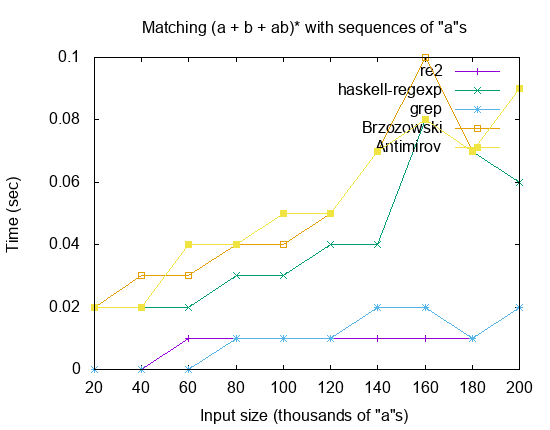
\includegraphics[width=0.7\textwidth]{as.png}
   \centering
   \caption{Results of experiment 1.}
   \label{fig:graph1}
\end{figure}

\begin{figure}[!ht]
    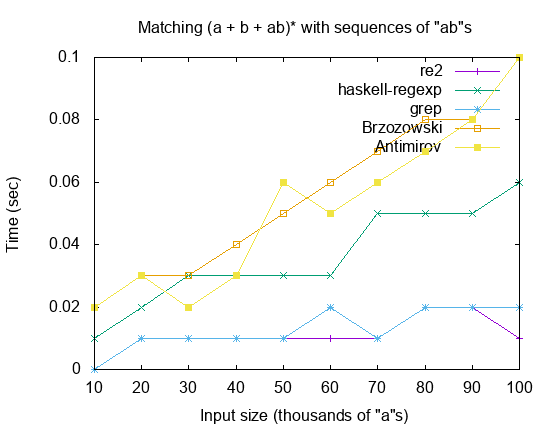
\includegraphics[width=0.7\textwidth]{abs.png}
   \centering
   \caption{Results of experiment 2.}
   \label{fig:graph2}
\end{figure}

Our tool behaves poorly when compared with all other options
considered. The cause of this inefficiency needs further
investigation, but we envisaged that it can be due to the
following: 1) Our algorithm relies on the Brzozowski's definition for RE
parsing, which needs to quotient resulting REs. 2) We use lists to
represent sets of Antimirov's partial derivatives. We believe that
usage of better data structures to represent sets and using
appropriate disambiguation strategies like greedy
parsing~\cite{FrischC04} and POSIX~\cite{SulzmannL14} would be able to
improve the efficiency of our algorithm without sacrificing
correctness. We leave the formalization of disambiguation strategies
and the use of more efficient data structures for future work.

\section{Related Work}\label{sec:related}

\paragraph{Parsing with derivatives} Recently, derivative-based
parsing has received a lot of attention. Owens et al. were the first
to present a functional encoding of RE derivatives and use it to
parsing and DFA building. They use derivatives to build scanner
generators for ML and Scheme~\cite{Owens2009}; no formal proof of
correctness was presented.

Might et al.~\cite{Might2011} report on
the use of derivatives for parsing not only RLs but also context-free
ones. He uses derivatives to handle context-free grammars (CFG) and
develops an equational theory for compaction that allows for efficient
CFG parsing using derivatives. Implementation of derivatives for CFGs
are described by using the Racket programming
language~\cite{Felleisen2013}. However, Might et al. do not present
formal proofs related to the use of derivatives for CFGs.

Fischer et al.~describe an algorithm for RE-based parsing based on
weighted automata in Haskell~\cite{Fischer2010}.  The paper describes
the design evolution of such algorithm as a dialog between three
persons. Their implementation has a competitive performance when
compared with Google's RE library~\cite{re2}. This work also does not
consider formal proofs of RE parsing.

An algorithm for POSIX RE parsing is described
in~\cite{SulzmannL14}. The main idea of the article is to adapt
derivative parsing to construct parse trees incrementally to solve
both matching and submatching for REs. In order to improve the
efficiency of the proposed algorithm, Sulzmann et al. use a bit
encoded representation of RE parse trees. Textual proofs of
correctness of the proposed algorithm are presented in an appendix.

\paragraph{Certified parsing algorithms} Certified algorithms for
parsing also received attention recently. Firsov et al.~describe a
certified algorithm for RE parsing by converting an input RE to an
equivalent NFA represented as a boolean matrix~\cite{FirsovU13}. A
matrix library based on some ``block'' operations~\cite{MacedoO13} is
developed and used Agda formalization of NFA-based parsing
~\cite{Norell2009}. Compared to our work, a NFA-based formalization requires
much more infrastructure (such as a Matrix library). No experiments
with the certified algorithm were reported.

Firsov describes an Agda formalization of a parsing algorithm that
deals with any CFG (CYK algorithm)~\cite{Firsov2014}. Bernardy
et al.~describe a formalization of another CFG parsing algorithm in
Agda~\cite{BernardyJ16}: Valiant's algorithm~\cite{Valiant1975}, which
reduces a CFG parsing problem to boolean matrix multiplication. In both works,
no experiment with formalized parsing algorithms were reported.

A certified LR(1) CFG validator is described
in~\cite{Jourdan2012}. The formalized checking procedure verifies if
a CFG and an automaton match. They proved soundness and completeness of
the validator in the Coq proof
assistant~\cite{Bertot2010}. Termination of the LR(1) automaton
interpreter is ensured by imposing a natural number bound on
allowed recursive calls.

Formalization of a parser combinator library was the subject of
Danielsson's work~\cite{Danielsson2010}. He built a library of parser
combinators using coinduction and provide correctness proofs of such
combinators.

Almeida et al.~\cite{AlmeidaMPS10} describe a Coq formalization of
partial derivatives and its equivalence with automata. Partial
derivatives were introduced by Antimirov~\cite{Antimirov91} as an
alternative to Brzozowski derivatives, since it avoids quotient
resulting REs with respect to ACUI axioms. Almeida et al. motivation
is to use such formalization as a basis for a decision procedure for
RE equivalence.

Ridge~\cite{Ridge2011} describes a formalization, in the HOL4 theorem
prover, of a combinator parsing library. A parser generator for such
combinators is described and a proof that generated parsers are sound
and complete is presented.  According to Ridge, preliminary results
show that parsers built using his generator are faster than those
created by Happy parser generator~\cite{Happy}.

Ausaf et. al.~\cite{AusafDU16} describe a formalization, in
Isabelle/HOL~\cite{Nipkow02}, of the POSIX matching algorithm proposed
by Sulzmann et.al.~\cite{SulzmannL14}. They give a constructive
characterization of what a POSIX matching is and prove that such
matching is unique for a given RE and string. No experiments with the
verified algorithm are reported.


\section{Conclusion}\label{sec:conclusion}

We gave a complete formalization of a derivative-based parsing
for REs in Agda. To the best of our knowledge, this is the first work
that presents a complete certification and that uses the certified
program to build a tool for RE-based search.

The developed formalization has 1145 lines of code, organized in 20
modules. We have proven 39 theorems and lemmas to complete the
development. Most of them are immediate pattern matching functions
over inductive datatypes and were omitted from this text for brevity.

As future work, we intend to work on the development of a certified
program of greedy and POSIX RE parsing using Brzozowski
derivatives~\cite{SulzmannL14,FrischC04} and investigate ways to
obtain a formalized but simple and efficient RE parsing tool.

\paragraph{Acknowledgements:} The first author thanks CNPq for financial
support. Second author thanks Fundação de Amparo a
Pesquisa de Minas Gerais (FAPEMIG) for financial support.

\section*{References}

\bibliography{main}

\end{document}
